%% SEGAN-D-26-03850, major revision.
%% An open curtailment dataset and a diagnostic for adaptive conformal
%% calibration under regime change.
%% Elsevier elsarticle template; compile with pdfLaTeX, three passes.
%% Table bodies are read with \input from the tab_*.tex and
%% hiperparametros.tex files that accompany this source.
\documentclass[preprint,3p,times]{elsarticle}

\usepackage{amsmath,amssymb,amsfonts}
\usepackage{graphicx}
\usepackage{booktabs}
\usepackage{url}
\usepackage[hidelinks]{hyperref}
\usepackage{siunitx}
\usepackage{multirow}
\usepackage{longtable}
\usepackage{algorithm}
\usepackage{algpseudocode}

\journal{Sustainable Energy, Grids and Networks}

\begin{document}

\begin{frontmatter}

\title{An open curtailment dataset and a diagnostic for adaptive conformal calibration under regime change}

\author[usach]{Pablo Reyes Cerda\corref{cor1}}
\ead{pablo.reyes.ce@usach.cl}
\author[ubb]{Kerven Cea Morales}
\ead{kceam@ubiobio.cl}

\cortext[cor1]{Corresponding author.}

\address[usach]{Mag\'ister en Gesti\'on de la Innovaci\'on y el Emprendimiento Tecnol\'ogico, Universidad de Santiago de Chile, Santiago, Chile}
\address[ubb]{Programa de Doctorado en Matem\'atica Aplicada, Universidad del B\'io-B\'io, Concepci\'on, Chile}

\begin{abstract}
Curtailment of variable renewable generation is zero-inflated, heavy-tailed and drifts as the system changes, a demanding target for calibrated uncertainty. We study it in Chile's National Electricity System, where roughly 19{,}000~GWh were curtailed between 2022 and mid-2026 and the distribution of magnitudes shifted. We contribute an open, plant-level, errata-corrected dataset of daily and hourly curtailment covering 53 continuous months (hydropower from June 2024) and 300 plants across four technologies, reconciling exactly with the operator's official annual totals; and a diagnostic. Paired with a zero-inflated lognormal base model, a scheme combining a probability-integral-transform score, score transport and online recalibration narrows the intervals of the most divergent window by about a third at near-nominal coverage. That gain does not survive a change of base model. On a multi-quantile gradient-boosting predictive fitted under the same protocol, the static conformal split is already at nominal coverage and the adaptive scheme returns slightly wider intervals. Across eight base models and five windows the width reduction grows with how much the static split over-covers ($r=-0.873$, bootstrap interval $[-0.912, -0.645]$; slope $-4.89$ per cent of width per percentage point), so the layer recovers base-model over-dispersion rather than distribution shift. Ablations agree: online adaptation earns its cost, score transport does not. Panel dependence is severe: intraclass correlation by date 0.238. We separate finite-sample marginal validity under exchangeability, long-run adaptive control, and empirical coverage in a dependent panel. The practical implication is that fixing the base predictive dominates fixing the calibration layer. Dataset and code are public.
\end{abstract}

\begin{keyword}
renewable curtailment \sep probabilistic forecasting \sep conformal prediction \sep distribution shift \sep model-agnostic evaluation \sep power system operations
\end{keyword}

\end{frontmatter}

%==================================================================
\section{Introduction}
\label{sec:intro}

The share of variable renewable energy has grown faster than the transmission and demand able to absorb it, and curtailment, the deliberate reduction of available solar, wind or hydropower output, has become a routine consequence of that imbalance rather than an exceptional event. O'Shaughnessy et al.~\cite{oshaughnessy2020} document the pattern across systems worldwide and show that solar curtailment rises sharply once penetration passes a threshold that varies by system but is reached quickly where network expansion lags. In Chile's National Electricity System (Sistema El\'ectrico Nacional, SEN), recorded curtailment rose from about 1.5~TWh in 2022 to more than 6~TWh per year by 2024, and the cumulative figure over 2022 to mid-2026 reaches roughly 19~TWh. For the owners of affected plants this is generated energy that is never remunerated; for the system it is a growing signal of the mismatch between where and when renewable energy is produced and where and when it can be used.

Anticipating curtailment is therefore of direct operational and commercial value, and it is considerably harder than forecasting generation. Generation depends primarily on weather and installed capacity, which are well understood and increasingly predictable. Curtailment depends on the state of the whole system: net load, transmission congestion, the marginal cost of energy and the behaviour of other assets. It is a downstream, system-level quantity, and this makes it both more difficult and less studied than generation forecasting.

Two features of the case at hand make it an informative test bed rather than merely an application. First, curtailment in the SEN is highly concentrated: a small number of northern regions, where solar capacity has outpaced the north-to-south transmission corridor, account for the large majority of national curtailment. Second, and central to this paper, the statistical distribution of curtailment changed materially over the study period. The change is gradual rather than abrupt: a formal change-point analysis of the monthly mean log-magnitude, described in Section~\ref{sec:data}, places the shift in a ramp of roughly eighteen months running from mid-2023 to late 2024, with no detected break in 2025 and none in October 2024. A model calibrated on one part of that trajectory is miscalibrated on a later part, not because the model is wrong but because the system it describes has changed. Two properties make the change a demanding case rather than a textbook one. It has no single identifiable cause: the growth of solar capacity behind a saturated corridor, the entry of battery storage, transmission reinforcements and changes in northern mining demand all act over the same months, and the data released here cannot separate them. And it is superimposed on a strong annual cycle, so that separating seasonal from secular movement is part of the problem: in the window where divergence from the calibration distribution is largest, the majority of the apparent jump turns out to be seasonal.

A further difficulty is that a point forecast of curtailment is of limited use for decision-making. Curtailment is zero-inflated and heavy-tailed: on a large fraction of days a given plant curtails nothing, and on the days it does the amounts vary widely. A single predicted number conveys neither the probability that curtailment will occur nor the range it might take. What a decision-maker needs is a calibrated statement of uncertainty. Providing such intervals, and keeping them informative when the system changes regime, is the problem we address.

This paper makes two contributions.

The first is a data contribution. We construct and release an open, plant-level dataset of curtailment in the SEN at daily and hourly resolution, spanning 53 continuous months and 300 plants across solar, wind and two hydropower technologies, built from the public reports of the system operator and reconciled against the official aggregate figures. In the course of building it we identified and corrected eight classes of errata in the original public files, using deterministic and reproducible rules, and recovered two calendar days missing from the operator's own daily breakdown. We are not aware of an open curtailment dataset at this granularity for a Latin American power system.

The second is a diagnostic contribution, and it is the one that changed most in the course of this work. Adaptive conformal calibration is the standard recommendation when exchangeability fails, and on this dataset it appears to deliver: paired with a two-part zero-inflated lognormal base model, a scheme that scores observations by their probability integral transform, transports the calibration scores onto the recent regime and wraps the result in an online update narrows the intervals of the most divergent window by about a third while holding coverage within one point of nominal. We show that this apparent success is not a property of the calibration layer. Repeating every experiment on a multi-quantile gradient-boosting predictive fitted on the same rows and features, with the same training cut-off, hyperparameters and seed, and calibrated with the same score, the same windows, the same seeds and the same embargo, the static conformal split already attains nominal coverage in the divergent window and the adaptive scheme returns intervals that are slightly \emph{wider}. Across eight base models and five evaluation windows, the width the adaptive layer recovers is linearly related to how much the static split over-covers. What the layer corrects, in this record, is over-dispersion of the base predictive, not distribution shift.

We take that finding seriously rather than burying it. Section~\ref{sec:results} reports it with its ablations, which localise the effect further: online adaptation is the component that earns its keep, score transport significantly \emph{worsens} the interval score once adaptation is present, and the bootstrap tail shrinkage that is the most intricate part of the construction improves it by eight tenths of one per cent while consuming most of the runtime. A one-sided conformalized quantile regression~\cite{romano2019}, a standard and far simpler construction, dominates the whole pipeline when paired with the better base model. We also treat the panel dependence of the data as a first-class problem rather than a caveat, and we separate three statements that are easy to conflate: the finite-sample marginal validity of the static split under exchangeability, the long-run coverage control of the adaptive update without exchangeability, and the empirical coverage actually observed in a dependent panel.

The remainder of the paper is organised as follows. Section~\ref{sec:related} reviews related work. Section~\ref{sec:data} describes the dataset and dates the distributional change. Section~\ref{sec:methods} presents the base forecasters, the conformal layer in full implementation detail, and the evaluation protocol. Section~\ref{sec:results} reports the empirical results. Section~\ref{sec:discussion} discusses what follows for practice, Section~\ref{sec:limitations} states the limitations, and Section~\ref{sec:conclusion} concludes.

%==================================================================
\section{Related work}
\label{sec:related}

This work sits at the junction of three literatures that rarely meet: the applied literature on curtailment and on the network constraints that cause it, the methodological literature on distribution-free uncertainty quantification, and the growing body of work on hybrid physical and data-driven modelling of power systems. We discuss each contribution individually rather than in groups, since what matters here is what each one establishes and where our problem departs from it.

\subsection{Curtailment: causes, measurement and forecasting}

Curtailment is best understood as the visible output of a constrained network rather than as a property of the plants that suffer it. Henriot~\cite{henriot2015} formalises the economically efficient level of curtailment and shows that some curtailment is optimal rather than a failure, which frames the forecasting problem as one of anticipating a rational system response. Joos and Staffell~\cite{joos2018} quantify the short-term integration costs of that response in Britain and Germany and show that curtailment and balancing costs are of comparable order, which is what makes anticipation commercially relevant. Tang et al.~\cite{tang2018} document the Chinese experience, where solar curtailment reached levels that triggered a national policy response, and attribute it primarily to transmission inadequacy rather than to oversupply as such. Schermeyer et al.~\cite{schermeyer2018} take the complementary view from the network side, showing on German distribution and transmission data how congestion management determines which plants are curtailed and when. Nycander et al.~\cite{nycander2020} extend the accounting to a whole synchronous area, decomposing Nordic curtailment into transmission capacity, inertia and flexibility limits, which is the closest published analogue to the concentrated, corridor-limited situation studied here. Yildiz et al.~\cite{yildiz2023} provide the counterpart at the other end of the system, using metered data from low-voltage networks to show how distributed photovoltaics and behind-the-meter storage are curtailed in practice, and how poorly that curtailment is captured by aggregate statistics.

Forecasting curtailment specifically, as opposed to explaining it, has received far less attention. Bunodiere and Lee~\cite{bunodiere2020} predict curtailment in Kyushu with a rule-based method built on the operator's own dispatch logic, which works where that logic is published and transferable and is difficult to generalise where it is not. The wider forecasting literature has instead treated curtailment as a nuisance term inside net-load forecasting, an approach that sidesteps the plant-level question a portfolio owner actually faces. Our problem differs from both: we forecast plant-level curtailment directly, at a seven-day horizon, without access to the operator's dispatch model, and we care about the uncertainty of that forecast rather than its point accuracy.

\subsection{Storage, congestion and network capacity as the physical drivers}

The physical mechanisms that generate curtailment matter here because they are the candidate explanations for the distributional change we document, and because they set the ceiling on what any forecast can know. Denholm and Mai~\cite{denholm2019} establish how much storage, and at what duration, is needed to absorb a given level of curtailment, a result that bounds how quickly storage entry can plausibly change a curtailment record. Wang et al.~\cite{wang2019} embed that question in unit commitment and show the trade-off between operating cost and wind curtailment when batteries participate in dispatch. Rayit et al.~\cite{rayit2021} evaluate the economics from the storage owner's side, treating curtailed wind as the input to a grid-services business. Mohamad et al.~\cite{mohamad2021} approach the same problem as one of siting rather than operation, optimising where storage should be placed on a network so as to minimise solar curtailment subject to power-flow constraints, which is the mechanism by which storage capacity in one region can fail to relieve curtailment in another.

On the network side, Vargas et al.~\cite{vargas2015} study wind curtailment and storage jointly as instruments of transmission congestion management, including plant ramp-rate limits, on a system with the same corridor-constrained geometry as the one considered here. Fang et al.~\cite{fang2021} characterise how locational marginal prices behave when renewable generation and demand are jointly uncertain, which is the price signal underlying the dispatch decisions that produce curtailment.

A distinct line of work attacks the constraint itself rather than its consequences, by rating network elements dynamically instead of conservatively. Foss et al.~\cite{foss1983} give the original dynamic ampacity algorithm, computing a conductor's real-time current-carrying capability from weather and thermal balance rather than from a fixed seasonal rating. Teh and Cotton~\cite{teh2016} show that applying dynamic thermal rating in a wind-integrated network changes system reliability, not only capacity, because the rating and the wind resource are correlated. Lai and Teh~\cite{lai2022} survey the field and set out where the practical limits lie. Glaum and Hofmann~\cite{glaum2023} quantify what dynamic line rating would deliver on the existing German transmission grid, and find capacity gains large enough to displace some network expansion. Su et al.~\cite{su2025} close the loop with our problem by forecasting short-term transmission capacity itself under dynamic line rating, which is the quantity that ultimately determines how much renewable output can be evacuated. For underground and cable-limited corridors the binding constraint is thermal rather than electrical: Maximov et al.~\cite{maximov2016} show how non-uniform soil temperature changes cable ampacity, and Ocło\'n~\cite{oclon2021} quantifies how soil thermal conductivity trades off against material cost in transmission design. We do not model any of these mechanisms. We cite them because they are the physical content of the shift our calibration layer has to survive, and because a forecaster with access to them would be solving a different and better-posed problem than ours.

\subsection{Hybrid physical and data-driven modelling}

The natural response to a data-driven model that drifts is to anchor it in physics. Lei et al.~\cite{lei2021} embed power-flow structure into a learned optimal power flow and show that the physical constraints act as a regulariser that improves extrapolation. Kruse et al.~\cite{kruse2023} apply the same idea to grid frequency, where the governing dynamics are known and the disturbances are not. Kirchner-Bossi et al.~\cite{kirchnerbossi2024} combine a physical wind-farm flow model with a data-driven correction for intra-day and day-ahead forecasting, and show the hybrid beats either component. This route is closed to us for a specific and instructive reason: the physics that determines curtailment is the operator's security-constrained dispatch, and neither the network model nor the constraint set is public. Our base model is therefore purely statistical by necessity, and that is precisely why the calibration layer has to carry the burden of the shift.

\subsection{Probabilistic forecasting and conformal prediction}

Probabilistic forecasting in power systems has largely converged on quantile methods. Maciejowska et al.~\cite{maciejowska2016} introduce factor quantile regression averaging for electricity prices and establish the benchmark that later work is measured against; Uniejewski and Weron~\cite{uniejewski2021} regularise it and show the gain is robust. Van der Meer et al.~\cite{vandermeer2018} study prediction intervals for solar power and net load and document how coverage degrades with aggregation level and penetration, which is the same conditional-coverage question we face across plants of different size. Mangalova and Shesterneva~\cite{mangalova2016} show that a nearest-neighbour construction is competitive in the GEFCom2014 probabilistic wind track, a useful reminder that simple non-parametric predictive distributions are hard to beat, and one our own benchmark results echo. None of these methods carries a finite-sample coverage guarantee.

Conformal prediction supplies one. Angelopoulos and Bates~\cite{angelopoulos2023} give the modern account: prediction sets with finite-sample, distribution-free marginal coverage under exchangeability, which is exactly the assumption a regime change violates. Two lines of work relax it. Tibshirani et al.~\cite{tibshirani2019} extend the guarantee to covariate shift by reweighting calibration points by a density ratio, which presupposes that the conditional law $\mathbb{P}(Y\mid X)$ is invariant and therefore fails when the change is in the conditional itself. Barber et al.~\cite{barber2023} dispense with exchangeability altogether, using fixed non-uniform weights and bounding the coverage gap in total variation, which covers the regime-change case directly but at the cost of a bound that is not computable from data. Gibbs and Cand\`es~\cite{gibbs2021} take the online route, updating the miscoverage level from observed errors to attain long-run coverage under arbitrary shifts, and their scheme is the adaptive component we use and ablate. Guan~\cite{guan2022} localises the calibration set around the test point, a different way of buying conditional validity that we do not pursue here but that is a natural competitor.

Two constructions are central to our implementation. Chernozhukov et al.~\cite{chernozhukov2021} score observations by their probability integral transform, which is what makes a score comparable across plants of very different size and what handles the atom at zero; our score is theirs. Romano et al.~\cite{romano2019} conformalize quantile regression directly, measuring nonconformity in the units of the response rather than in probability, and their method is the benchmark that turns out to dominate our own pipeline in Section~\ref{sec:results}. Applications of these ideas to power systems are recent and growing. Hu et al.~\cite{hu2022} conformalize a temporal convolutional quantile network for wind power intervals, and Jensen et al.~\cite{jensen2024} show that ensembling conformalized quantile regressors improves both coverage and sharpness for time series. Neither addresses regime change, and neither, to our knowledge, asks the question this paper turns out to be about: how much of the benefit attributed to a calibration layer is really an artefact of the base model it is correcting.

Three further tools are used rather than extended. Peyr\'e and Cuturi~\cite{peyre2019} give the computational treatment of optimal transport from which we take the monotone one-dimensional map. Chernozhukov et al.~\cite{chernozhukov2010} establish that rearranging a set of estimated quantile curves into a monotone one is never worse in an appropriate sense, which is what licenses the rearrangement step in our multi-quantile base model. Killick et al.~\cite{killick2012} give the PELT algorithm used to date the distributional change, and Gneiting and Raftery~\cite{gneiting2007} give the theory of proper scoring rules from which our evaluation metric is derived.

%==================================================================
\section{Data}
\label{sec:data}

\subsection{Source and scope}

The dataset consolidates the curtailment records published monthly by Chile's National Electricity Coordinator (Coordinador El\'ectrico Nacional, CEN) into two validated relational tables. The daily table contains 293{,}678 records and the hourly table 6{,}906{,}761 records, both covering the continuous period from 1 January 2022 to 31 May 2026, that is 1{,}612 days built from all 53 monthly reports, with no missing days. Records span 300 generation plants across four technologies: solar photovoltaic (75 plants), wind (56), run-of-river hydropower (140) and reservoir hydropower (29). Twelve hydropower plants are labelled inconsistently across the operator's monthly reports, alternating between the run-of-river and reservoir categories; the plant registry resolves each of them to a single canonical technology, so that a count of distinct plant-technology pairs in the raw daily table returns 312 rather than 300. Hydropower curtailment records are present from June 2024 onward, with hourly hydropower detail from July 2024, following the coverage of the underlying public reports.

Each plant is linked to a metadata registry matched to the CEN installation catalogue, with 18 fields including the official identifier, installed capacity, owner, region, province, municipality, geographic coordinates, commissioning date, connection point and regulatory classification; the matching method is recorded for every plant. Days and hours without curtailment are stored explicitly as zero-valued records, which represent 49.8\% of daily and 83.6\% of hourly rows. This explicit encoding of zeros is deliberate: it preserves the zero-inflated structure of the quantity, which is essential for the modelling in Section~\ref{sec:methods}. Figure~\ref{fig:map} shows the geographic distribution of the plants, with the concentration of solar capacity in the northern regions and of hydropower in the south.

\begin{figure}[tp]
\centering
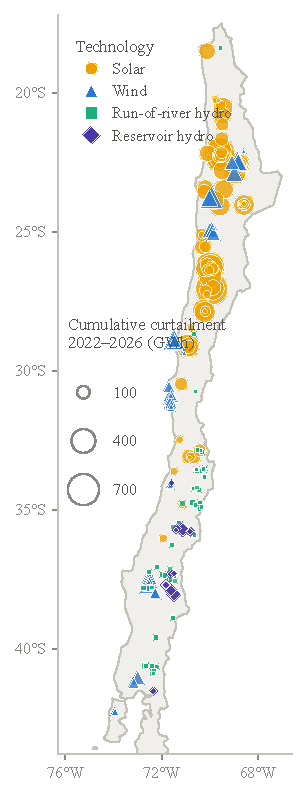
\includegraphics[width=0.45\textwidth]{fig1_plants_map.pdf}
\caption{Geographic distribution of the 300 power plants in the dataset, coloured and shaped by technology, with marker area proportional to each plant's cumulative curtailed energy over January 2022 to May 2026.}
\label{fig:map}
\end{figure}

\subsection{Construction and validation}

The 53 monthly reports were retrieved from the CEN public portal with a versioned download script, parsed and loaded into a relational database, and the original files were preserved unmodified with SHA-256 checksums. During construction we identified eight classes of errata in the original publications. Five were corrected or recovered deterministically in the curated tables and three are limitations of the source that we document without correction. Among the corrections, two omitted calendar days were recovered from the corresponding monthly hourly sheets and cross-checked to the millesimal against the source files' own total columns; one of these was detectable only by a structural continuity check, since the omitted day carried zero energy and was therefore invisible to any energy-based validation.

Two independent checks establish the fidelity of the result. Annual totals from the daily table match the CEN official summary exactly, to a difference of 0.000~GWh, in every year from 2022 to 2026, and aggregate 2022 wind and solar curtailment reproduces the 1.47~TWh independently reported by Fraunhofer Chile for that year. At monthly resolution the agreement is close but not exact: in a census month-by-month reconciliation of hourly sums against daily totals over all 53 months, 50 months agree within 1\% and 35 agree exactly, while the three remaining months correspond to documented inconsistencies within the operator's own publications. The residual sub-percent differences arise from the operator reassigning the same monthly energy differently across sister run-of-river units between its monthly hourly sheets and its annual closing, with a net effect of zero at system level, which is the same mechanism as errata classes six and seven. The dataset totals 19{,}030~GWh of recorded curtailment over the period.

The dataset is publicly available on Zenodo under a CC~BY~4.0 licence~\cite{dataset2026}, together with the data dictionary, the errata log and the integrity checksums. The processing pipeline that regenerates every curated table is available in the companion code repository.

\subsection{Exploratory characterisation}
\label{sec:eda}

Three features of the data govern the modelling choices that follow.

First, curtailment is strongly zero-inflated and its occurrence is persistent in time, with a daily lag-one autocorrelation of roughly 0.85 at system level and a marked weekly cycle. Second, the positive magnitudes are heavy-tailed and approximately lognormal, with a ratio between the 99th and 50th percentiles of the order of twenty-five across technologies, and of about fifteen for solar alone. Figure~\ref{fig:dist} illustrates both.

\begin{figure}[tp]
\centering
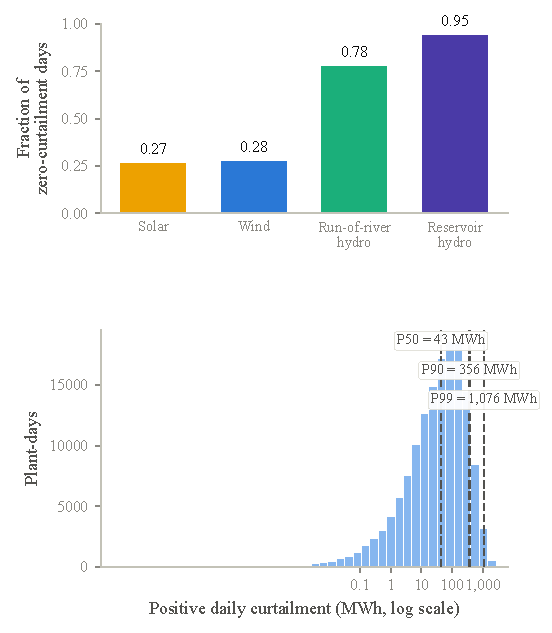
\includegraphics[width=0.75\textwidth]{fig2_distribution.pdf}
\caption{Distributional structure of plant-level curtailment. Top: share of zero-valued plant-days by technology. Bottom: distribution of positive magnitudes on a logarithmic scale, with the 50th, 90th and 99th percentiles marked. The combination of a large point mass at zero and a heavy right tail motivates the two-part model of Section~\ref{sec:methods}.}
\label{fig:dist}
\end{figure}

Third, the change in the distribution of curtailment over the study period acts on scale, not on occurrence and not on timing. Occurrence is stable: for solar plants in the northern regions the probability of a positive day, averaged over each evaluation window, stays between 0.750 and 0.815 from January 2024 to May 2026, and a change-point search on the monthly series of $\mathbb{P}(Y>0)$ returns no break after September 2022. At monthly resolution the same series ranges more widely, from 0.635 to 0.877, so the stability claim is one about window aggregates and not about individual months. The intraday shape is nearly as stable: the peak hour of the normalised intraday profile is hour 16 in every half-year from 2022 to the first half of 2025 and hour 17 in the last two half-years, two adjacent hours whose profile masses differ by less than 0.4 percentage points; the centroid of the profile moves by at most 22 minutes between consecutive half-years after 2023-H1, and the total variation distance between the profiles of consecutive half-years stays between 0.032 and 0.079 over the same span. The positive magnitudes, in contrast, roughly triple: the median of positive daily curtailment for solar plants in Antofagasta and Atacama rises from 92~MWh in the calibration window to 267~MWh in October to December 2024. These three facts, zero inflation, heavy tails and a scale-type shift, motivate respectively the two-part model, the choice of evaluation metric and the adaptive calibration described next.

\subsection{Dating the distributional change}
\label{sec:regime}

The timing of the change in scale is best read after removing the annual cycle. Figure~\ref{fig:regime} shows the monthly mean of $\log Y$ over positive plant-days for solar plants in Antofagasta and Atacama, together with the same series net of a calendar-month median. Applied to the deseasonalised series with the PELT algorithm of Killick et al.~\cite{killick2012} and with binary segmentation, both under an $L_2$ cost and a BIC penalty $\hat\sigma^2\log n$ with a minimum segment length of three months, the two algorithms return two breaks and agree on both: May 2023, with a jump of $+1.05$ in mean log-magnitude, and January 2024, with a jump of $+0.76$. Neither returns a break in October 2024, and neither returns any break in 2025.

That conclusion is robust to the analyst's choices. Repeating the detection over 180 configurations, crossing two strata, three deseasonalisation methods (calendar-month median, calendar-month mean and a robust STL decomposition), five penalty multipliers and three minimum segment lengths, no configuration returns a break in 2025 and none returns a break in October 2024. The change is therefore a ramp of roughly eighteen months rather than a step, and it is essentially complete by the end of 2024: comparing like with like across years, the Wasserstein-1 distance between the positive log-magnitudes of October to December 2023 and those of October to December 2024 is 1.20, whereas between October to December 2024 and October to December 2025 it is 0.085, below the 0.115 threshold of a permutation null that resamples whole days and therefore not distinguishable from no change at all.

\begin{figure*}[tp]
\centering
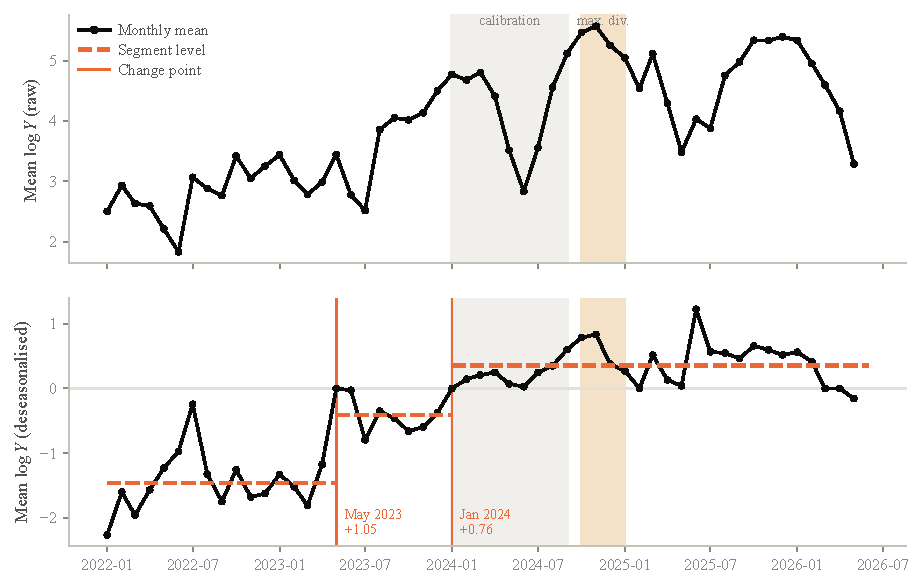
\includegraphics[width=\textwidth]{fig5_regime_changepoints.pdf}
\caption{Monthly mean of $\log Y$ over positive plant-days, solar plants in Antofagasta and Atacama. Top: raw series, dominated by the austral annual cycle. Bottom: the same series net of a calendar-month median, with the two change points returned by PELT and by binary segmentation marked by vertical lines (May 2023 and January 2024) and the calibration and transition windows of Section~\ref{sec:methods} shaded. Neither algorithm returns a break in October 2024 or in 2025; the deseasonalised level reaches its maximum in October and November 2024 and then stops rising. The isolated spike of June 2025, discussed in Section~\ref{sec:discussion}, is the largest deseasonalised anomaly of the post-calibration record.}
\label{fig:regime}
\end{figure*}

Because the annual cycle is strong, any contrast between windows that fall in different seasons registers a large distance even when no regime change is present, and this bears directly on how the evaluation windows of Section~\ref{sec:methods} should be read. Table~\ref{tab:seasonal} decomposes the January--September to October--December shift in the monthly mean of $\log Y$ into a seasonal component, given by the calendar-month effects and therefore identical in every year, and a secular remainder. In 2024 the shift is the largest of the record, but 61\% of it for northern solar, and 76\% at system level, is the seasonal component that recurs every year; the same contrast yields a Wasserstein-1 distance of 0.96 in 2023 and 0.88 in 2025, years for which no regime change is claimed. The secular remainder of 2024, $+0.46$ for northern solar, is real and is the largest of the four years, but it is of the same order as the $+0.29$ of 2023. We report the raw contrast throughout the results, and flag here that it should not be read as if it were entirely a regime effect.

%% generated by flagship/revision/fase9_tablas_tex.py from resultados/
%% do not edit by hand
\begin{table}[t]
\centering
\caption{Decomposition of the January--September to October--December shift in the monthly mean of $\log Y$ over positive plant-days, in log units, by year. The seasonal component is the difference between the calendar-month effects of the two windows and is by construction the same in every year; the secular component is the remainder. The 2024 row is the contrast that defines the transition window used in the evaluation; the final row of each block repeats the decomposition on the calibration window itself (January to August against October to December 2024), which is the pair the evaluation actually uses. Generated from \texttt{resultados/fase6/fase6\_descomposicion\_estacional.csv}.}
\label{tab:seasonal}
\begin{tabular}{lcccc}
\toprule
Year & Total shift & Seasonal & Secular & Seasonal share \\
\midrule
\multicolumn{5}{l}{\emph{Solar, Antofagasta and Atacama}} \\
\quad 2022 & $+0.64$ & $+0.72$ & $-0.09$ & 113\% \\
\quad 2023 & $+1.01$ & $+0.72$ & $+0.29$ & 72\% \\
\quad \textbf{2024} & $\mathbf{+1.18}$ & $\mathbf{+0.72}$ & $\mathbf{+0.46}$ & 61\% \\
\quad 2025 & $+0.90$ & $+0.72$ & $+0.17$ & 81\% \\
\quad 2024, calibration window & $+1.29$ & $+0.78$ & $+0.50$ & 61\% \\
\addlinespace
\multicolumn{5}{l}{\emph{System (solar and wind)}} \\
\quad 2022 & $+0.77$ & $+0.66$ & $+0.11$ & 86\% \\
\quad 2023 & $+0.89$ & $+0.66$ & $+0.23$ & 74\% \\
\quad \textbf{2024} & $\mathbf{+0.86}$ & $\mathbf{+0.66}$ & $\mathbf{+0.20}$ & 76\% \\
\quad 2025 & $+0.71$ & $+0.66$ & $+0.05$ & 93\% \\
\quad 2024, calibration window & $+0.94$ & $+0.69$ & $+0.24$ & 74\% \\
\bottomrule
\end{tabular}

\vspace{3pt}
\parbox{\linewidth}{\footnotesize Note: the calendar-month effects are estimated as the median of each calendar month over the whole record. A robust STL decomposition returns somewhat different values on a 53-month series carrying a strong trend; it does not change the order of magnitude of the split, and the secular components remain the smaller part of the 2024 contrast.}
\end{table}


%==================================================================
\section{Methods}
\label{sec:methods}

\subsection{Problem setup and base forecasters}
\label{sec:base}

For each plant $i$ and target day $T$ we forecast the curtailed energy $Y_{iT}\ge 0$ from information available at the forecast origin $t=T-7$, a direct seven-day-ahead formulation. The feature vector $x_{iT}$ has twelve components: the most recent observation $y_{i,t}$, three lags $y_{i,t-1}$, $y_{i,t-7}$ and $y_{i,t-14}$, seven- and thirty-day trailing means ending at $t$, an occurrence indicator $\mathbb{1}\{y_{i,t}>0\}$, the day of week and day of year of the target, the log of installed capacity, and the region and technology as categorical variables. Every dynamic feature is a shift of at least seven days on a calendar-continuous index, which is verified by assertion at construction time and rules out leakage by design. All base models are fitted on targets up to 31 December 2023 and never see the evaluation period; hyperparameters were fixed a priori and were not tuned against it.

The paper uses three base predictives, which differ only in the shape they impose on $\mathbb{P}(Y\mid x)$.

\emph{Hurdle with constant dispersion.} The base model of the submitted version, and the reference throughout. It factorises the predictive into occurrence and magnitude,
\begin{equation}
Y \mid x \;\sim\; \big(1-p(x)\big)\,\delta_0 \;+\; p(x)\,\mathrm{LogNormal}\big(\mu(x),\sigma^2\big),
\label{eq:hurdle}
\end{equation}
with $p(x)$ from a gradient-boosting classifier and $\mu(x)$ from a gradient-boosting regression on $\log y$ over positive days. The dispersion $\sigma$ is estimated out of fold, by five-fold cross-fitting on the training period, to avoid the downward bias of the in-sample residual variance of a boosted model; on these data $\hat\sigma=1.70$, which we return to in Section~\ref{sec:results} because it sets the sharpness floor of the whole pipeline.

\emph{Hurdle with conditional dispersion.} The same construction with $\sigma$ replaced by a fitted $\sigma(x)$, estimated out of fold from the squared stage-one residuals with a global scale correction and a floor at the fifth percentile of the training distribution. It is included to separate two possible explanations of the results: that the difficulty lies in the constant dispersion, or that it lies in the lognormal shape itself.

\emph{Multi-quantile gradient boosting.} A predictive defined not by a parametric family but by a dense grid of 54 estimated quantiles, at levels 0.02 to 0.98 in steps of 0.02 plus 0.005, 0.01, 0.99, 0.995 and 0.999, fitted with the pinball loss under exactly the same features, rows, training cut-off, per-model hyperparameters and seed as the hurdle. One thing this does not hold fixed is capacity. The hurdle is two boosted models, a classifier and a regressor; the multi-quantile predictive is 54 boosted models of 400 trees each, one per quantile level. Matching the training protocol is not the same as matching the number of fitted parameters; Section~\ref{sec:escalera} separates the two experimentally and Section~\ref{sec:limitations} states what the separation does and does not licence. Estimated quantile curves may cross, and we restore monotonicity by rearrangement in the sense of Chernozhukov et al.~\cite{chernozhukov2010}, sorting each row and clipping at zero. Two properties matter for what follows. The predictive CDF is the interpolated inverse of the quantile function, so it is not committed to any tail shape. And the mass at zero is not imposed: it is read off the grid as $F_x(0)=\max\{\tau_k:\hat q_{\tau_k}(x)=0\}$, so zero inflation emerges from the fit rather than from the model form. Beyond the highest estimated level the predictive expresses nothing, so a requested quantile above $\tau=0.999$ returns $+\infty$ and is counted as an infinite interval under the same rule applied to every other method.

This third model exists because of a specific question, raised in review and taken up in Section~\ref{sec:agnostic}: whether the behaviour of the calibration layer is a property of the layer or of the predictive it is wrapped around.

\subsection{Conformal calibration with a PIT score}
\label{sec:pit}

A point forecast, or even the raw predictive, does not by itself guarantee that a stated interval contains the realised value with the nominal probability. We obtain that guarantee by conformal calibration. Rather than measuring nonconformity in energy units, which are not comparable across plants of very different size, we score each observation by its probability integral transform under the predictive law,
\begin{equation}
s \;=\; F_x(y),
\label{eq:pit}
\end{equation}
following the distributional-conformal construction of Chernozhukov et al.~\cite{chernozhukov2021}. Because $F_x$ has an atom at zero, the score is randomised there in the standard way for mixed distributions~\cite{smith1985}: for $y=0$ we set $s=F_x(0^-)+U\big(F_x(0)-F_x(0^-)\big)$ with $U\sim\mathrm{Uniform}(0,1)$, which for the hurdle reduces to $s=(1-p(x))\,U$; for $y>0$ no randomisation is needed. Under the true predictive law $s$ is then $\mathrm{Uniform}(0,1)$, and it lives on a common $[0,1]$ scale across plants of any size, which is why it handles the atom and the plant heterogeneity cleanly. The same two operations, the CDF and its generalised inverse, are all the calibration layer ever asks of the base model, and this is what makes the comparison of Section~\ref{sec:agnostic} exact rather than approximate: the three predictives are substituted behind an identical interface.

For the hurdle this score has a further property that motivated the transport step. For a positive observation the score is a monotone transform of the standardised log-magnitude $z=(\log y-\mu(x))/\sigma$, namely $s=(1-p)+p\,\Phi(z)$. A change of scale of the magnitude distribution by a factor $c$ is a location shift $\log c$ of $\log Y$, hence a translation of $z$ by $\delta=\log c/\sigma$. It is therefore a translation on the latent Gaussian scale, and only a monotone displacement of the law of $s$ on $[0,1]$; it is not a translation of $s$ itself. This low-dimensional structure, established under the empirically supported assumption that the shift rescales the positive magnitudes while leaving occurrence and intraday timing essentially unchanged (Section~\ref{sec:eda}), is what suggested that the displacement could be estimated from a short recent window while the shape of the tail is inherited from the large calibration set. That structure is a property of the base model rather than of the data: the single translation $\delta=\log c/\sigma$ exists because the hurdle models every positive magnitude as lognormal with one dispersion $\sigma$, so the motivation for the transport holds for the hurdle only. Under the conditional-dispersion hurdle the translation varies with $x$, and under the multi-quantile predictive the displacement of each score depends on the shape of its own estimated distribution, so for the other two base models of Section~\ref{sec:agnostic} the transport is the same algorithm without that motivation.

Given a calibration set of size $n$ scored by~\eqref{eq:pit}, the conformal quantile is the order statistic $\hat q=s_{(k)}$ with $k=\lceil (n+1)(1-\alpha)\rceil$, which yields the finite-sample marginal guarantee $\mathbb{P}(Y \le U(x)) \ge 1-\alpha$ under exchangeability; when $k>n$ the quantile is $+\infty$ and the interval is the whole line. For the hurdle the upper prediction limit $U(x)=F_x^{-1}(\hat q)$ is recovered in closed form: it is zero when $\hat q\le 1-p(x)$, it is $+\infty$ when $\hat q\ge 1$, and otherwise
\begin{equation}
U(x) \;=\; \exp\!\Big(\mu(x) + \sigma\,\Phi^{-1}\!\big(\textstyle\frac{\hat q-(1-p(x))}{p(x)}\big)\Big).
\label{eq:invert}
\end{equation}
A short proof of the inversion is given in \ref{app:inversion}, and it was additionally checked numerically against oracle coverage. For the multi-quantile predictive the same inversion is a linear interpolation on the quantile grid.

\subsection{Three guarantees, and which one applies where}
\label{sec:guarantees}

It is easy, and consequential, to conflate three statements that this paper keeps separate.

\emph{Finite-sample marginal validity.} The static split satisfies $\mathbb{P}(Y\le U(x))\ge 1-\alpha$ exactly, at the stated $n$, provided the calibration scores and the test score are exchangeable. This is a statement about an average over draws of the whole calibration set and the test point, not about any particular plant, day or window.

\emph{Long-run adaptive control.} The online update of Gibbs and Cand\`es~\cite{gibbs2021} guarantees $\frac1T\sum_{t\le T}\mathrm{err}_t\to\alpha$ for \emph{any} sequence, with no distributional assumption whatever. It says nothing about coverage at any finite time, and in exchange it discards the finite-sample guarantee of the split.

\emph{Empirical coverage in this panel.} What we actually measure. Neither of the two statements above describes it, because exchangeability fails here twice over, and not only across the regime boundary. All plants share the daily state of the system, so the calibration scores arrive in strongly correlated daily blocks. We quantify this rather than assert it. On the calibration set, the intraclass correlation of the PIT score by date is 0.238, and with 108.8 plants per day this gives a design effect of 26.7: the effective calibration sample is about 1{,}000 rows, not the 26{,}552 that the finite-sample guarantee would nominally be stated at. Every coverage figure we report therefore carries a standard error clustered by date, and every difference between methods carries a bootstrap interval that resamples whole days. Section~\ref{sec:panel} tests calibration schemes designed to restore exchangeability at the block, group and plant level, and reports how far each one actually moves conditional coverage.

\subsection{Responses to the shift}
\label{sec:respuestas}

We consider four responses, of which the last is the one the submitted version proposed.

\emph{Weighted conformal.} Reweighting each calibration point by an estimate of the density ratio between calibration and test distributions is the standard remedy for \emph{covariate} shift~\cite{tibshirani2019}. It is the wrong tool here: the shift changes the conditional law $\mathbb{P}(Y\mid x)$, not the marginal of $x$, so no reweighting of old scores can reflect the new conditional, and the density-ratio estimate degenerates because features that are monotone in time separate calibration from test almost perfectly. On a synthetic panel where covariate shift can be isolated, the per-point implementation returns infinite intervals for a large fraction of test points (\texttt{flagship/conformal\_v2.py} in the companion repository); we report this as a negative result about the tool that motivates the alternatives. We take instead the fixed-recency-weight scheme of Barber et al.~\cite{barber2023} as the recency benchmark, in its simplest form: the sliding window below, which gives weight one to the scores of the most recent 60 days before the embargo and zero to all earlier ones.

\emph{Sliding-window recalibration.} We discard old calibration data and recalibrate on a trailing 60-day window refreshed every 7 days. Because the base model forecasts at a 7-day horizon, the label of an origin is realised only 7 days later; to avoid using information unavailable at the forecast origin, every online calibration window ends 7 days before its target. We call this the horizon embargo and it applies to every online method. The static split does not use online calibration and is therefore unaffected, which serves as an implementation control.

\emph{Adaptive conformal inference.} We update the effective miscoverage level online~\cite{gibbs2021}, $\alpha_{t+1}=\alpha_t+\gamma(\alpha-\mathrm{err}_t)$ with $\mathrm{err}_t=\mathbb{1}\{Y_t>U_t\}$ averaged over the plants of day $t$, where the error feedback is delayed by the same 7-day embargo.

\emph{Transport of scores.} Motivated by the monotone-displacement structure of Section~\ref{sec:pit}, we transport the calibration scores from the old regime onto the new one before conformalising. Let $\hat F_{\mathrm{old}}$ and $\hat F_{\mathrm{new}}$ be the empirical CDFs of the calibration scores and of the scores in the recent window; the monotone one-dimensional optimal-transport map is the increasing rearrangement $T=\hat F_{\mathrm{new}}^{-1}\circ\hat F_{\mathrm{old}}$~\cite{peyre2019}, estimated nonparametrically by interpolation between empirical quantiles. In the upper tail, where the short window is noisy, the map is shrunk towards the identity in proportion to a bootstrap estimate of its variance, so that a noisy new quantile is replaced by the stable old one rather than extrapolated. Because the transport map is data-dependent it breaks the exchangeability of the transported scores with the test score; we therefore restore validity operationally by wrapping the transported scores in the online adaptive scheme, so that coverage is controlled by the adaptive update and the transport contributes only sharpness. An idealised validity argument, exact under an oracle map and controlled through the total-variation framework of Barber et al.~\cite{barber2023} under an estimated map, is given in \ref{app:coverage}.

\subsection{The adaptive scheme in full}
\label{sec:algoritmo}

The construction above is stated at the level of ideas. Because reproducibility of the exact procedure is the point, Algorithm~\ref{alg:transporte} gives it completely, Figure~\ref{fig:flow} shows the data flow, and \ref{app:hiper} tabulates every constant, including the seeds. Three implementation choices deserve to be stated in the body because they are the ones a reader would otherwise have to guess.

\emph{The quantile grid and the interpolation.} The map is estimated on an equispaced grid of $g$ probability levels on $[0,1]$, with $g=\min(100,\max(20,m/2))$ where $m$ is the number of scores in the recent window; the second term prevents a grid finer than the data supports. The map is applied by two successive linear interpolations, first from a score to its level on the old empirical quantile function, then from that level to the regularised new quantile, which is exactly the increasing rearrangement evaluated pointwise.

\emph{The shrinkage function and its strength.} The recent window is bootstrapped $B=150$ times; the map is the mean of the $B$ replicate quantile functions, which is a bagged estimate, and the replicate standard deviation $\mathrm{sd}_{\mathrm{boot}}(u)$ at each level $u$ is the width of the uncertainty band. The regularised quantile is
\begin{equation}
\hat q_{\mathrm{reg}}(u)=\big(1-\lambda(u)\big)\,\hat q_{\mathrm{old}}(u)+\lambda(u)\,\hat q_{\mathrm{new}}^{\mathrm{bag}}(u),
\qquad
\lambda(u)=\frac{1}{1+\big(\mathrm{sd}_{\mathrm{boot}}(u)/\tau\big)^2},
\label{eq:shrink}
\end{equation}
with $\tau=0.05$ in PIT units, a fixed regularisation scale that was never tuned against the test set. Where the bootstrap is stable $\lambda\approx1$ and the map transports fully; where it is noisy $\lambda\approx0$ and the map reverts to the identity, that is to the stable old quantile. The result is monotonised by a running maximum and clipped to $[0,1]$ so that it remains a quantile function.

\emph{The order of execution.} On date $t$: (i) if a refresh is due, the map is recomputed from the recent window ending at $t-7$ and the entire calibration pool is transported; (ii) the conformal quantile is taken from the transported pool at the \emph{current} $\alpha_t$, which does not yet incorporate the error of day $t$; (iii) the interval is emitted; (iv) the error of day $t$ enters the embargo queue and updates $\alpha$ only seven steps later. The map never uses the adaptive level and the adaptive update never uses the map; the sole coupling between the two branches is the pool they share.

\begin{figure*}[tp]
\centering
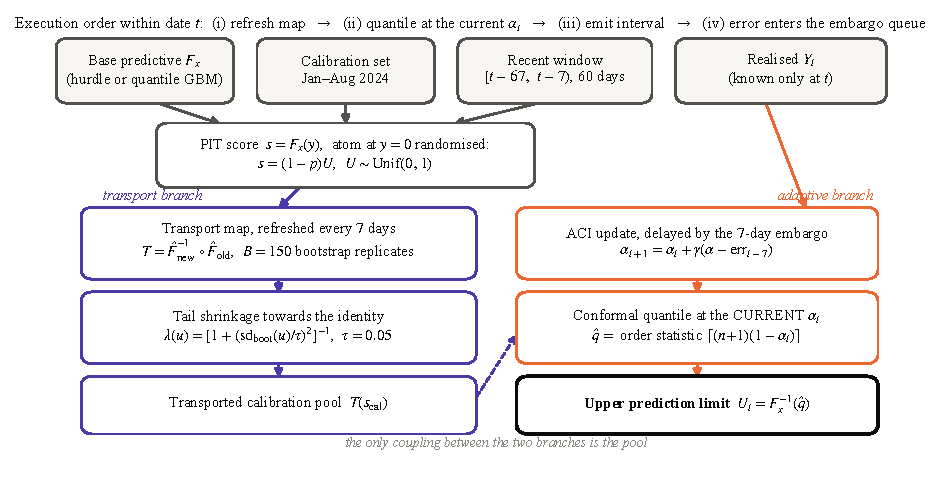
\includegraphics[width=\textwidth]{fig6_algorithm_flow.pdf}
\caption{Data flow of the adaptive scheme, from the base predictive to the upper prediction limit. The transport branch (left) estimates and regularises the map; the adaptive branch (right) maintains the effective miscoverage level. The two are coupled only through the transported calibration pool, and the order of operations within a date is stated at the top: the conformal quantile is taken at the level in force before the day's own error is observed, and that error is fed back only after the seven-day horizon embargo.}
\label{fig:flow}
\end{figure*}

\begin{algorithm}[t]
\caption{Transport + ACI with tail shrinkage. Constants and seeds in \ref{app:hiper}.}
\label{alg:transporte}
\begin{algorithmic}[1]
\Require base predictive $F_x$; calibration scores $s_{\mathrm{cal}}$ of size $n$; nominal level $\alpha$; step $\gamma$; window $W$; refresh period $R$; embargo $E$; bootstrap size $B$; shrinkage scale $\tau$
\State $\alpha_1\gets\alpha$; \; $\mathcal{P}\gets\mathrm{sort}(s_{\mathrm{cal}})$; \; queue $\mathcal{Q}\gets\emptyset$; \; $t_{\mathrm{next}}\gets t_0$
\For{each test date $t$}
  \If{$t\ge t_{\mathrm{next}}$}
     \State $s_{\mathrm{new}}\gets$ scores with date in $[t-W-E,\;t-E)$
     \If{$|s_{\mathrm{new}}|\ge 100$}
        \State draw $B$ bootstrap resamples of $s_{\mathrm{new}}$; set $\hat q^{\mathrm{bag}}_{\mathrm{new}}$ to their mean quantile function and $\mathrm{sd}_{\mathrm{boot}}$ to its replicate standard deviation
        \State form $\hat q_{\mathrm{reg}}$ by~\eqref{eq:shrink}; monotonise by running maximum; clip to $[0,1]$
        \State $T\gets$ interpolation from $\hat q_{\mathrm{old}}$ to $\hat q_{\mathrm{reg}}$; \; $\mathcal{P}\gets\mathrm{sort}\big(T(s_{\mathrm{cal}})\big)$
     \EndIf
     \State $t_{\mathrm{next}}\gets t+R$
  \EndIf
  \State $k\gets\lceil (n+1)(1-\alpha_t)\rceil$; \; $\hat q_t\gets \mathcal{P}_{(k)}$ if $k\le n$, else $+\infty$
  \State $U_t\gets F_x^{-1}(\hat q_t)$ for every plant of date $t$ \Comment{interval emitted here}
  \State push $\mathrm{err}_t=\frac{1}{|I_t|}\sum_{i\in I_t}\mathbb{1}\{Y_{it}>U_{it}\}$ onto $\mathcal{Q}$
  \If{$|\mathcal{Q}|>E$}
     \State pop $\mathrm{err}_{t-E}$ from $\mathcal{Q}$; \; $\alpha_{t+1}\gets\mathrm{clip}\big(\alpha_t+\gamma(\alpha-\mathrm{err}_{t-E}),\;\alpha_{\min},\;\alpha_{\max}\big)$
  \EndIf
\EndFor
\end{algorithmic}
\end{algorithm}

\subsection{What is new here, and what is not}
\label{sec:novedad}

Every ingredient of Algorithm~\ref{alg:transporte} is taken from existing work, and it is worth being exact about which.

The probability-integral-transform score is the distributional-conformal score of Chernozhukov et al.~\cite{chernozhukov2021}; the randomisation of the atom for a mixed distribution is the classical device of Smith~\cite{smith1985}. The online update of the miscoverage level is the adaptive conformal inference of Gibbs and Cand\`es~\cite{gibbs2021}, unmodified. The monotone one-dimensional transport map is the increasing rearrangement, standard in optimal transport~\cite{peyre2019} and, in the quantile-curve setting, the rearrangement of Chernozhukov et al.~\cite{chernozhukov2010}. Bagging a bootstrap estimate and shrinking it towards a stable reference in proportion to its variance is ordinary shrinkage practice.

What is new is the combination and one specific device. The combination is applying a transport of the \emph{score} distribution, rather than of the response or the covariates, as a sharpness-only step inside an online adaptive scheme that carries the coverage control, so that the data-dependence of the map cannot damage validity. The device is the variance-proportional tail shrinkage~\eqref{eq:shrink}, which uses the bootstrap dispersion of the estimated map to interpolate between transporting and not transporting, level by level.

The two fare differently under ablation, and Section~\ref{sec:ablaciones} reports both outcomes. The combination does not survive: once the online update is in place, adding the transport \emph{worsens} the interval score by 68.6~MWh over the whole test, with an interval that excludes zero. The device does survive, but not its price: the variance-proportional shrinkage improves the interval score by 6.4~MWh, with a bootstrap interval that also excludes zero, for eight tenths of one per cent of the score and ninety-one per cent of the runtime. We regard stating both plainly as more useful than the claim of novelty they replace.

\subsection{Hyperparameter selection}
\label{sec:seleccion}

The submitted version reported the adaptive methods at $\gamma\in\{0.02,0.05\}$ with a 60-day window, values taken from a synthetic prototyping stage and from common practice rather than from a formal selection on real data. That does not meet the standard the results should be held to, so the selection was redone.

Base-model predictions exist only from 1 January 2024, since the base models are trained through 2023, so the only material available before the test period is the 244-day calibration window. We split it: January to April 2024 becomes an inner calibration pool and May to August 2024 an inner validation set, evaluated in rolling origin with the same seven-day refresh and seven-day embargo as the real protocol. The selection criterion is the mean interval score of Section~\ref{sec:evaluacion}, which is proper, is in MWh, and takes the value $+\infty$ if the configuration produces any infinite interval, so that a configuration escaping into uninformative intervals is disqualified by the criterion itself rather than by an ad hoc rule. The grids are $\gamma\in\{0.005,0.01,0.02,0.05,0.10,0.20\}$ and window lengths $\{30,45,60,90,120\}$ days.

The selection returns $\gamma=0.005$ for pure adaptive conformal inference and $\gamma=0.005$ with a 120-day window for the transported variant. Both are an order of magnitude gentler than the values reported in the submitted version, and both produce no infinite intervals at all in validation, whereas at $\gamma=0.05$ between 34 and 42 per cent of validation intervals are infinite. The test set was not used in the selection and is used once, for the final evaluation. Sensitivity over the full $6\times5$ grid is reported on the test set in Section~\ref{sec:frontera}, Table~\ref{tab:sens_hiper}, as a display, never as a criterion, and we say so there.

\subsection{Evaluation}
\label{sec:evaluacion}

The forecasts are upper prediction limits, that is one-sided intervals $[0,U(x)]$ at level $1-\alpha=0.90$, and the evaluation has to be appropriate to that. We report empirical coverage against the nominal level with standard errors clustered by date, and, for sharpness, the mean width over finite intervals together with the fraction of infinite ones. Reporting only those two, as the submitted version did, is misleading in a specific way: a method that escapes into infinite intervals removes its widest cases from the width average and therefore looks sharper for having failed. Some configurations here produce close to 10 per cent infinite intervals in 2025-S1 and 2025-S2, so this is not a hypothetical concern.

Our primary metric is therefore the interval score of the one-sided limit $[0,U]$ at level $1-\alpha$, which follows from the scoring rules of Gneiting and Raftery~\cite{gneiting2007} for the quantile of that level,
\begin{equation}
\mathrm{IS}_\alpha(U,y) \;=\; U \;+\; \frac{1}{\alpha}\,\max(y-U,\,0).
\label{eq:is}
\end{equation}
The multiplier is $1/\alpha$ and not the $2/\alpha$ of the central interval score: in a one-sided limit all of the mass $\alpha$ lies in the upper tail, whereas the central interval places $\alpha/2$ in each tail, and with $2/\alpha$ the score would be minimised by the quantile of level $1-\alpha/2$ rather than by the one every method calibrates. It is proper, it is in MWh, it penalises width and non-coverage on the same scale, and it is $+\infty$ whenever $U$ is, so it cannot be improved by escaping. We report it in two forms and label them: $\mathrm{IS}$ restricted to finite intervals, which is comparable across methods but incomplete, and the unrestricted mean, which is the verdict and is infinite for any method that produces even one infinite limit. We also report the continuous ranked probability score of the base predictive and the Brier score of the event $\{Y>0\}$; both are properties of the base model rather than of the calibration layer, which is precisely why they cannot arbitrate between calibration schemes and why the interval score is needed.

Differences between methods are reported with a bootstrap interval that resamples whole days, 2{,}000 replicates, since the day is the unit of dependence in this panel. Coverage is reported both marginally and conditionally, by technology, capacity tercile, region, and on high-curtailment days, defined as those above the ninetieth percentile of system-level daily curtailment in the calibration window.

The calibration set is January to August 2024. The first test month is September 2024. The following window, October to December 2024, is the transition window on which the calibration layer is stressed, and it is selected as the window of maximum divergence from the calibration distribution, not as the interval of entry of any particular technology: measured by the Wasserstein-1 distance between the positive log-magnitudes of each test window and those of the calibration set, it scores 1.25 against 0.28 to 0.95 for the other four windows. That distance is almost entirely a displacement of location: the change is close to a pure translation of the distribution of log-magnitudes, and for a pure translation the Wasserstein-1 distance equals the difference in means, the two agreeing to within 0.001 for this contrast. Carried out on the calibration window itself, the seasonal decomposition of Table~\ref{tab:seasonal} splits that displacement 61 per cent seasonal for northern solar and 74 per cent at system level. On that basis the window is best understood as the hardest case the calibration layer faces in this record, not as the signature of a single event, and Section~\ref{sec:frontera} shows that the conclusions do not depend on where exactly its boundaries are drawn. The remaining periods are taken by semester. The base forecaster is benchmarked against persistence, a seasonal-naive predictor, a point gradient-boosting model and a quantile gradient-boosting model.

%==================================================================
\section{Results}
\label{sec:results}

\subsection{Point forecasting adds little, within the scope tested}
\label{sec:punto}

Table~\ref{tab:mae} reports the mean absolute error of the base models on the out-of-sample period. The seasonal-naive predictor, which averages the same weekday over recent weeks, is the most accurate of all and is not beaten by the gradient-boosting models; the hurdle mixture median, which is optimised for the full predictive law rather than for absolute error, is the least accurate on this metric. This ordering follows from the strong weekly persistence documented in Section~\ref{sec:eda}: when a quantity is that persistent, sophisticated point models add little over a well-chosen calendar rule.

The scope of that conclusion should be stated precisely, because it is easy to over-read. It holds for these five model classes, this twelve-feature set, this seven-day horizon and mean absolute error as the criterion. It does not establish that point forecasting of curtailment is generally of little value. A model with access to the operator's network model, to weather forecasts, to unit-commitment schedules or to the storage state of charge would be solving a better-posed problem, and a criterion other than mean absolute error, in particular one that weighted the large-magnitude days that carry the economic mass, might well order these same models differently. What the table supports is narrower and still operationally useful: within the information set available to a plant owner from public data, effort is better spent on quantifying uncertainty than on refining the predicted number.

One robustness check belongs here, because Section~\ref{sec:escalera} reports that the hurdle used throughout this paper is not the best available on this problem. Refitting it with early stopping, which selects 105 trees and improves its CRPS by 5.7 per cent, worsens its mean absolute error from 104.1 to 108.6~MWh and would place it last in this table, 27.6 per cent behind the seasonal-naive predictor. The ordering here is therefore not an artefact of the particular hurdle we fitted. It is also a measured instance of the criterion-dependence noted above: the two fits are ordered one way by a proper scoring rule of the whole predictive and the other way by point accuracy, because the early-stopped fit is the wider and better-calibrated predictive and its conditional median sits further from the realised value. We draw nothing further from it.

%% generated by flagship/revision/fase9_tablas_tex.py from resultados/
%% do not edit by hand
\begin{table}[t]
\centering
\caption{Mean absolute error (MWh) of the base forecasters on the out-of-sample period, on the common row set. Lower is better. The comparison is between these model classes on this feature set at this horizon under this criterion; see the scope statement in the text. Computed from \texttt{flagship/predicciones/}.}
\label{tab:mae}
\begin{tabular}{lcccc}
\toprule
Model & 2024 & 2025 & 2026 & Total \\
\midrule
Seasonal-naive (weekly) & 84.3 & 86.3 & 84.2 & 85.1 \\
Multi-quantile GBM (median) & 87.7 & 89.0 & 84.1 & 87.6 \\
Quantile GBM, 3 levels (median) & 88.5 & 89.9 & 84.3 & 88.3 \\
Persistence & 88.4 & 96.3 & 90.7 & 92.2 \\
Point XGBoost & 92.7 & 94.6 & 89.7 & 93.0 \\
Hurdle (mixture median) & 104.4 & 104.8 & 101.6 & 104.1 \\
\bottomrule
\end{tabular}
\end{table}


\subsection{With the hurdle base model, the shift inflates intervals and adaptation recovers them}
\label{sec:hurdle}

On real data the shift does not break coverage; it inflates it. Under a static conformal split with the hurdle predictive, empirical coverage stays between 89\% and 95\% in every period (Table~\ref{tab:results}), so the severe over-coverage seen on synthetic data is absent, because the base forecaster, through its lagged and moving-average features, absorbs much of the shift into its own predictive. The cost of the shift is paid in width rather than in coverage, and it is concentrated in the transition window: the static split reaches 95.3\% coverage with a mean width of 1203~MWh during October to December 2024. Part of that widening is seasonal rather than secular, in the proportion given in Table~\ref{tab:seasonal}, and the same qualitative pattern would be expected in the fourth quarter of any year in this record; what distinguishes 2024 is that the seasonal peak lands on top of the largest secular displacement of the four years. Figure~\ref{fig:rolling} traces the behaviour over time: the static split drifts above the nominal level as the window advances, while the adaptive schemes track it more closely.

\begin{figure*}[t]
\centering
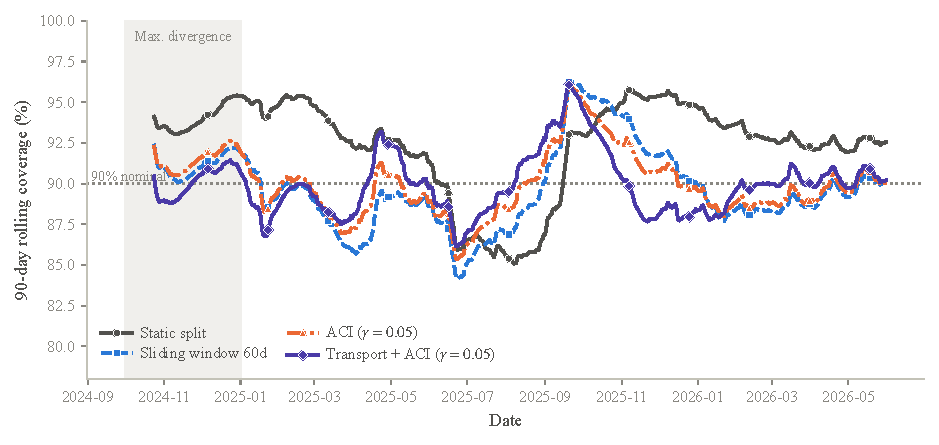
\includegraphics[width=\textwidth]{fig3_rolling_coverage.pdf}
\caption{Rolling empirical coverage (90-day window) of the conformal methods on real data with the hurdle base model, computed with the 7-day horizon embargo. The dashed line marks the 90\% nominal level and the shaded band marks the window of maximum divergence from the calibration distribution, October to December 2024. The static split drifts into over-coverage as that window advances, whereas the adaptive schemes remain close to nominal.}
\label{fig:rolling}
\end{figure*}

The adaptive schemes pay off precisely there. Transport of the calibration scores wrapped in online adaptation ($\gamma=0.05$) brings the transition intervals down to 806~MWh at 90.9\% coverage, a reduction of about a third at a coverage within one point of nominal, and the sliding window gives 834~MWh at 92.0\%. Outside that window the trade-off is ambiguous: with the static split already near nominal, the adaptive methods mostly exchange coverage for width and can under-cover, as in 2025-S1, and their gains are small and within the date-clustered standard error. That is what the data predict rather than a shortcoming of the adaptive layer. The first semester of 2025 is not distinguishable from the pre-transition regime: the Wasserstein-1 distance between the positive log-magnitudes of January to September 2024 and those of January to June 2025 is 0.1722, with a 95\% bootstrap interval of $[0.0703,0.3665]$ resampling whole days, against a threshold of 0.1931 under a permutation null that also resamples whole days. There is no shift left to correct in that period.

%% generated by flagship/revision/fase9_tablas_tex.py from resultados/
%% do not edit by hand
\begin{table*}[t]
\centering
\footnotesize
\caption{Coverage and mean interval width of the conformal methods by period, on real data with the hurdle base model, with the 7-day horizon embargo. Each cell shows coverage in percent (clustered standard error by date in parentheses) over mean interval width in MWh. Nominal coverage is 90\%. The base-model CRPS is a property of the predictive, not of the calibration layer, and is reported once per period. Superscripts give the fraction of infinite intervals where nonzero; Section~\ref{sec:metricas} reports the metric that does not let those cases improve a method's score. Generated from \texttt{flagship/conformal\_v3\_tabla.csv}.}
\label{tab:results}
\begin{tabular}{l@{\hspace{5pt}}c@{\hspace{5pt}}c@{\hspace{5pt}}c@{\hspace{5pt}}c@{\hspace{5pt}}c}
\toprule
Method & test\_pre & test\_transition & 2025-S1 & 2025-S2 & 2026-S1 \\
 & (Sep 24, stable) & (Oct--Dec 24, max.\ divergence) & & & \\
\midrule
Static split (PIT) & 93.5\,(1.03) / 799 & 95.3\,(0.45) / 1203 & 89.4\,(1.04) / 455 & 94.0\,(0.45) / 750 & 92.5\,(0.58) / 535 \\
Sliding window 60d & 93.0\,(1.04) / 742 & 92.0\,(0.73) / 834 & 85.4\,(1.16) / 323 & 92.9\,(0.51) / 650 & 89.5\,(0.76) / 419 \\
ACI ($\gamma{=}0.02$) & 93.0\,(1.06) / 759 & 93.5\,(0.55) / 915 & 85.7\,(1.16) / 345 & 93.5\,(0.49) / 669 & 89.1\,(0.76) / 405 \\
ACI ($\gamma{=}0.05$) & 92.4\,(1.16) / 718 & 92.1\,(0.67) / 822 & 86.6\,(1.14) / 405\textsuperscript{2.8} & 92.5\,(0.58) / 609\textsuperscript{11.8} & 89.8\,(0.75) / 446 \\
Transport+ACI ($\gamma{=}0.02$) & 92.6\,(1.07) / 713 & 91.1\,(0.8) / 787 & 86.5\,(1.17) / 437\textsuperscript{0.6} & 92.4\,(0.6) / 986\textsuperscript{1.1} & 90.3\,(0.73) / 459 \\
Transport+ACI ($\gamma{=}0.05$) & 92.0\,(1.19) / 681 & 90.9\,(0.81) / 806 & 87.4\,(1.13) / 446\textsuperscript{9.9} & 91.6\,(0.63) / 718\textsuperscript{10.7} & 90.5\,(0.72) / 489 \\
\midrule
Base-model CRPS (MWh) & 96.1 & 133.5 & 70.5 & 94.5 & 79.0 \\
\bottomrule
\end{tabular}
\end{table*}


\begin{figure*}[t]
\centering
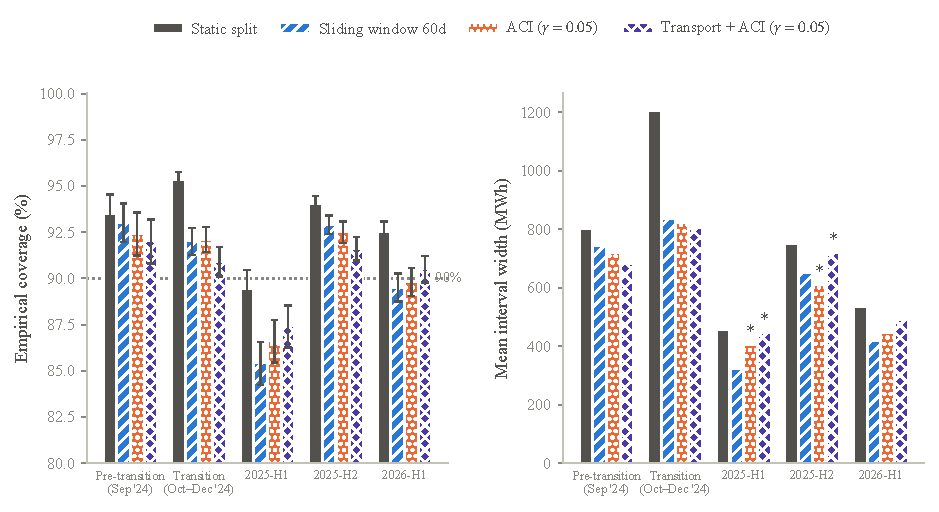
\includegraphics[width=\textwidth]{fig4_coverage_width.pdf}
\caption{Coverage and sharpness by method and period, hurdle base model. Left: empirical coverage with date-clustered standard errors against the 90\% nominal level. Right: mean interval width. Asterisks mark bars whose mean width is computed over finite intervals only, because the corresponding configuration returns at least 1\% of infinite intervals.}
\label{fig:tradeoff}
\end{figure*}

Read on its own, this subsection is the result the submitted version reported. The next one is why we no longer read it on its own.

\subsection{The gain does not survive a change of base model}
\label{sec:agnostic}

The calibration layer touches the base model through exactly two operations, the predictive CDF and its inverse, so the same layer can be run over a different predictive without changing a single constant. We do that, holding fixed the score, the window boundaries, the seven-day embargo, the seeds, the values of $\gamma$, the 60-day recent window and the tail shrinkage, and varying only the base model among the three of Section~\ref{sec:base}. As a control on the comparison, the hurdle arm of this experiment reproduces Table~\ref{tab:results} in all thirty cells and four metrics, which is verified by assertion inside the script that produces it. Any difference between arms is therefore attributable to the base model and not to the protocol. \emph{Base model} here means the pair (functional form, capacity) jointly: the arms differ both in the shape imposed on the predictive and in the number of boosted models fitted, and this design does not separate the two. That matters for the comparison of levels, and Section~\ref{sec:escalera} separates them; it does not affect the diagnostic relationship, which is established \emph{within} each arm by contrasting the static split against the adaptive scheme under one and the same predictive.

Table~\ref{tab:agnostic} gives the result in the transition window and Figure~\ref{fig:agnostic} summarises it. The reduction of about a third disappears. With the conditional-dispersion hurdle the static split already sits at 91.7\% and the adaptive scheme recovers only 4.8\% of width while dropping to 89.5\% coverage. With the multi-quantile predictive the static split is at 90.6\% coverage with a mean width of 410~MWh, and the adaptive scheme returns intervals 3.6\% \emph{wider}, at 425~MWh. The bootstrap interval of that width difference over whole days is $+15.1$~MWh with a 95\% interval of $[+0.0,+30.3]$, which only just excludes zero, and the corresponding difference in interval score, $+14.5$ with an interval of $[+4.9,+24.0]$, also excludes it. On either reading the point estimate is on the opposite side from the one reported, and the reduction is absent.

%% generated by flagship/revision/fase9_tablas_tex.py from resultados/
%% do not edit by hand
\begin{table*}[t]
\centering
\footnotesize
\caption{The same calibration layer over three base predictives, transition window (October to December 2024), nominal 90\%. Coverage in percent with date-clustered standard error, mean width in MWh over finite intervals, interval score of the one-sided limit in MWh restricted to finite intervals, fraction of infinite intervals, and base-model CRPS in MWh. Only the base model differs across blocks; the score, the windows, the embargo, the seeds and every constant of the calibration layer are identical. Generated from \texttt{resultados/fase0/fase0\_tabla\_por\_modelo.csv}.}
\label{tab:agnostic}
\begin{tabular}{lccccc}
\toprule
Method & Coverage (se) & Width & Interval score & \% infinite & CRPS \\
\midrule
\multicolumn{6}{l}{\emph{Hurdle, constant $\sigma$}} \\
\quad Static split (PIT) & 95.3\,(0.45) & 1203 & 1395 & 0.0 & 133.5 \\
\quad Sliding window 60d & 92.0\,(0.73) & 834 & 1112 & 0.0 & 133.5 \\
\quad ACI ($\gamma{=}0.02$) & 93.5\,(0.55) & 915 & 1158 & 0.0 & 133.5 \\
\quad ACI ($\gamma{=}0.05$) & 92.1\,(0.67) & 822 & 1096 & 0.0 & 133.5 \\
\quad Transport+ACI ($\gamma{=}0.02$) & 91.1\,(0.8) & 787 & 1089 & 0.0 & 133.5 \\
\quad Transport+ACI ($\gamma{=}0.05$) & 90.9\,(0.81) & 806 & 1107 & 0.0 & 133.5 \\
\addlinespace
\multicolumn{6}{l}{\emph{Hurdle, $\sigma(x)$}} \\
\quad Static split (PIT) & 91.7\,(0.63) & 770 & 992 & 0.0 & 125.0 \\
\quad Sliding window 60d & 88.7\,(0.88) & 627 & 932 & 0.0 & 125.0 \\
\quad ACI ($\gamma{=}0.02$) & 89.9\,(0.77) & 657 & 928 & 0.0 & 125.0 \\
\quad ACI ($\gamma{=}0.05$) & 89.5\,(0.82) & 649 & 927 & 0.0 & 125.0 \\
\quad Transport+ACI ($\gamma{=}0.02$) & 88.9\,(0.94) & 669 & 969 & 0.0 & 125.0 \\
\quad Transport+ACI ($\gamma{=}0.05$) & 89.5\,(0.96) & 733 & 1000 & 0.0 & 125.0 \\
\addlinespace
\multicolumn{6}{l}{\emph{Quantile GBM}} \\
\quad Static split (PIT) & 90.6\,(0.85) & 410 & 588 & 0.0 & 92.9 \\
\quad Sliding window 60d & 90.1\,(0.94) & 409 & 598 & 0.0 & 92.9 \\
\quad ACI ($\gamma{=}0.02$) & 90.6\,(0.86) & 412 & 588 & 0.0 & 92.9 \\
\quad ACI ($\gamma{=}0.05$) & 90.6\,(0.87) & 412 & 588 & 0.0 & 92.9 \\
\quad Transport+ACI ($\gamma{=}0.02$) & 90.4\,(0.98) & 420 & 601 & 0.0 & 92.9 \\
\quad Transport+ACI ($\gamma{=}0.05$) & 90.5\,(0.99) & 425 & 602 & 0.0 & 92.9 \\
\bottomrule
\end{tabular}
\end{table*}


\begin{figure*}[t]
\centering
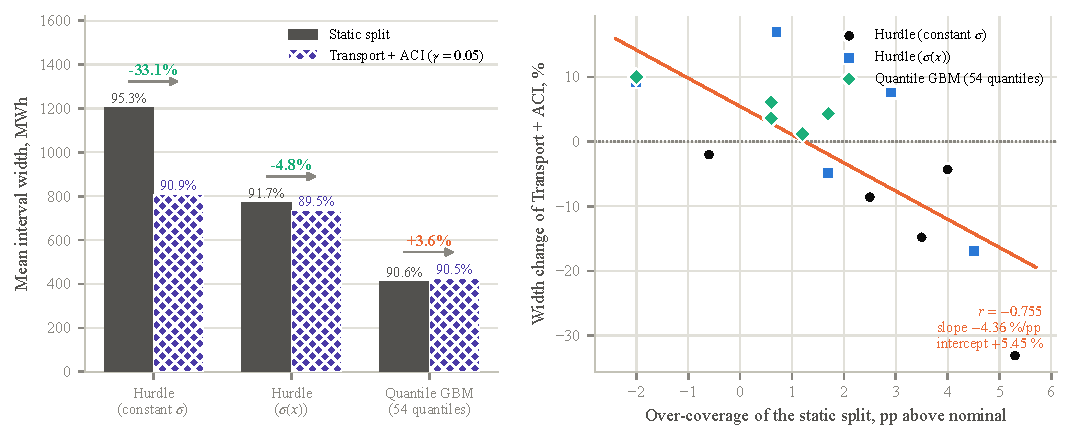
\includegraphics[width=\textwidth]{fig7_model_agnostic.pdf}
\caption{Left: mean interval width in the transition window for the static split and for Transport+ACI, by base model, with empirical coverage above each bar (nominal 90\%) and the width change marked by the arrow. Right: the diagnostic. Over the fifteen cells given by three base models and five evaluation windows, the width change achieved by Transport+ACI is linearly related to how far above nominal the static split sits in that cell. When the static split is already at nominal the adaptive layer costs width rather than saving it.}
\label{fig:agnostic}
\end{figure*}

The pattern is not confined to the transition window, and it is systematic. Table~\ref{tab:diagnostico} lays out all fifteen cells given by three base models and five windows. The width change achieved by the adaptive layer is linearly related to how far above nominal the static split sits in the same cell, with a Pearson correlation of $-0.755$ and a slope of $-4.36$ per cent of width per percentage point of over-coverage. The intercept is $+5.45$ per cent: when the static split is already at the nominal level, the adaptive layer makes intervals about five per cent wider. That is the diagnostic. What the layer recovers is not distributional displacement; it is the over-dispersion the base model built into every interval, and the size of the apparent gain is a measurement of how badly the base model was calibrated in the first place.

%% generado por flagship/revision/fase9_tablas_tex.py
%% NO EDITAR A MANO: se regenera desde resultados/
\begin{table*}[t]
\centering
\footnotesize
\caption{The diagnostic, over the fifteen cells given by three base models and five evaluation windows. Over-coverage is the coverage of the static split minus the 90\% nominal level. The width change is that of Transport+ACI ($\gamma=0.05$) relative to the static split in the same cell. Generated from \texttt{resultados/fase0/fase0\_diagnostico.csv}.}
\label{tab:diagnostico}
\begin{tabular}{lcccc}
\toprule
Window & Static coverage (\%) & Over-coverage (pp) & Static width (MWh) & Width change (\%) \\
\midrule
\multicolumn{5}{l}{\emph{Hurdle, constant $\sigma$}} \\
\quad Sep '24 & 93.5 & +3.5 & 799 & -14.8 \\
\quad Oct--Dec '24 & 95.3 & +5.3 & 1203 & -33.1 \\
\quad 2025-S1 & 89.4 & -0.6 & 455 & -2.0 \\
\quad 2025-S2 & 94.0 & +4.0 & 750 & -4.3 \\
\quad 2026-S1 & 92.5 & +2.5 & 535 & -8.6 \\
\addlinespace
\multicolumn{5}{l}{\emph{Hurdle, $\sigma(x)$}} \\
\quad Sep '24 & 94.5 & +4.5 & 662 & -16.9 \\
\quad Oct--Dec '24 & 91.7 & +1.7 & 770 & -4.8 \\
\quad 2025-S1 & 88.0 & -2.0 & 366 & +9.2 \\
\quad 2025-S2 & 92.9 & +2.9 & 584 & +7.6 \\
\quad 2026-S1 & 90.7 & +0.7 & 414 & +16.9 \\
\addlinespace
\multicolumn{5}{l}{\emph{Quantile GBM}} \\
\quad Sep '24 & 91.2 & +1.2 & 326 & +1.2 \\
\quad Oct--Dec '24 & 90.6 & +0.6 & 410 & +3.6 \\
\quad 2025-S1 & 88.0 & -2.0 & 221 & +10.0 \\
\quad 2025-S2 & 91.7 & +1.7 & 319 & +4.3 \\
\quad 2026-S1 & 90.6 & +0.6 & 253 & +6.1 \\
\midrule
\multicolumn{5}{l}{Pearson $r = -0.757$; slope $-4.39$ \% of width per pp of over-coverage; intercept $+5.49$ \%} \\
\bottomrule
\end{tabular}
\end{table*}


The relationship can be estimated on more than these fifteen cells. Each arm of the capacity ladder of Section~\ref{sec:escalera} was run through the same calibration layer in the same five windows, so eight base models are available rather than three, giving forty cells. We exclude the coarse-grid arm discussed in Section~\ref{sec:limitations}, whose static split returns infinite limits throughout and therefore yields no width. The addition matters for a specific reason: the fifteen cells span over-coverage only over $[-2.06, +5.34]$ percentage points, and the low-capacity arms reach $-8.42$, filling the region below nominal where the three-model design has no point at all and on which the intercept depends.

%% generated by flagship/revision/fase9_tablas_tex.py from resultados/
%% do not edit by hand
\begin{table*}[t]
\centering
\footnotesize
\caption{The diagnostic relationship over the forty cells given by eight base models and five evaluation windows, with 95\% bootstrap intervals resampling whole days, common to all cells, 2{,}000 replicates, seed 20260901. The restriction to the fifteen cells of the three-model design of Table~\ref{tab:diagnostico} is shown for comparison, as is the fit over the 25 cells in which the static split over-covers, the region to which the claim is scoped, with intervals from the same replicates. Generated from \texttt{resultados/fase0b/fase0b\_diagnostico.json}.}
\label{tab:diag_ampliado}
\begin{tabular}{lccc}
\toprule
& Pearson $r$ & Slope (\%/pp) & Intercept (\%) \\
\midrule
Fit over all 40 cells & $-0.873$ & $-4.89$ & $+5.76$ \\
\quad 95\% bootstrap interval & $[-0.912, -0.645]$ & $[-5.62, -3.30]$ & $[+1.60, +9.84]$ \\
\addlinespace
Restricted to the 15 cells of the three-model design (Table~\ref{tab:diagnostico}) & $-0.755$ & $-4.36$ & $+5.45$ \\
\addlinespace
Restricted to the 25 cells in which the static split over-covers & $-0.870$ & $-6.97$ & $+11.97$ \\
\quad 95\% bootstrap interval & $[-0.928, -0.528]$ & $[-7.90, -3.60]$ & $[+3.06, +17.07]$ \\
\addlinespace
Range of over-coverage covered & \multicolumn{3}{c}{$[-8.42, +5.34]$ pp over 40 cells, against $[-2.06, +5.34]$ over 15} \\
Leave-one-cell-out range of $r$ & \multicolumn{3}{c}{$[-0.889, -0.820]$} \\
Leave-one-base-model-out range of $r$ & \multicolumn{3}{c}{$[-0.899, -0.792]$} \\
\bottomrule
\end{tabular}
\end{table*}


Table~\ref{tab:diag_ampliado} reports the result and Figure~\ref{fig:escalera} shows it. The relationship strengthens: $r$ goes from $-0.755$ to $-0.873$ and the slope from $-4.36$ to $-4.89$ per percentage point. The bootstrap intervals, computed by resampling whole days once per replicate and recomputing all forty cells on that resample so that the crossed dependence between arms and windows is preserved, exclude zero for all three statistics, and the intercept, which on fifteen cells was $[+0.07, +11.25]$ and barely excluded zero, is now $[+1.60, +9.84]$. Leaving out any single cell moves $r$ within $[-0.889, -0.820]$, and leaving out any entire base model within $[-0.899, -0.792]$, so no arm carries the result.

One qualification belongs here. Fitting the two sides of the nominal level separately improves the residual sum of squares by more than chance ($F(2,36)=6.778$, $p=0.0032$), so we do not state the relationship symmetrically. The improvement is one of level and not of rate: allowing the intercept alone to differ accounts for it ($F(1,37)=12.982$, $p=0.0009$) and allowing the slope to differ as well adds nothing ($F(1,36)=0.685$, $p=0.413$). The rate at which the adaptive layer converts a departure from nominal coverage into width is the same on both sides, $-6.50$ per percentage point; what differs is the offset. We therefore keep the claim scoped to over-coverage, which is the region the three-model design covers densely, and record the under-covered arms as evidence that the mechanism does not stop at the nominal level rather than as a symmetric law. Restricted to the twenty-five cells in which the static split over-covers, the region to which the claim is scoped, the slope is steeper, $-6.97$ with a bootstrap interval of $[-7.90, -3.60]$ against $-4.89$ over all forty cells, and the relationship keeps its sign and its strength, $r=-0.870$, $[-0.928, -0.528]$ (Table~\ref{tab:diag_ampliado}); the figures quoted in the abstract are those of all forty cells.

We probed that break rather than accepting it, because the obvious worry is that one arm carries it. Of the 15 cells below nominal, 5 come from the lowest-capacity quantile arm, and 3 of the 4 cells below $-2$ percentage points come from the same arm. Removing it does not remove the break: on the remaining 35 cells the level shift grows from $-11.80$ to $-13.59$ per cent and the statistic rises rather than falls. Dropping any single arm leaves the shift between $-10.63$ and $-13.59$. Absorbing a separate intercept for each base model, so that the break is identified only from variation within arms, leaves it at $-11.48$ per cent. The break is not the artefact of one arm.

It is, however, an artefact of the specification in a different sense, and this is what decides the wording. Fitting the 35 cells without the extreme arm and predicting that arm out of sample, the specification with a break predicts its most extreme cell almost exactly, $+54.2$ against $+55.7$ observed where the single line predicts $+43.0$, but it is worse on the other four, and the out-of-sample root mean squared error ends up a tie, 8.85 against 8.82. A quadratic term tells the same story from the other side: it is indistinguishable from zero over the forty cells ($p=0.71$) and strongly significant over the thirty-five ($F(1,32)=27.9$). A design whose preferred functional form flips when one arm is removed does not determine that form, and the honest conclusion is that these data locate the relationship but not its shape below nominal. That is the reason we do not generalise the claim, and it is a stronger reason than the break statistic alone.

These $F$ tests treat the forty cells as independent observations, which they are not: they come in blocks of five per base model and eight per window and share the underlying panel, so the $p$ values are optimistic. We report them only as grounds for \emph{not} widening the claim, a direction in which optimistic $p$ values are conservative. The intervals that govern the statements this paper does make are the day-block bootstraps of Table~\ref{tab:diag_ampliado}.

Two further observations sharpen the reading. First, the multi-quantile predictive is not merely different, it is better on every proper metric and in every window: its CRPS is 18 to 30 per cent lower than the hurdle's, 92.9 against 133.5~MWh in the transition window, an advantage that Section~\ref{sec:escalera} decomposes into a contribution of the model form and one of the fitted budget, and the best of the eighteen model-by-method combinations by interval score is the multi-quantile predictive in all five windows, in four of them paired with the plain static split and no adaptive layer at all. Its intervals in the transition window are 410~MWh at 90.6\% coverage, against 806~MWh at 90.9\% for the full pipeline of the submitted version. Second, the hurdle retains one advantage that should be recorded: the Brier score of the occurrence event is better under the hurdle, 0.0721 against 0.1027 in the transition window. That comparison is not like for like, since the occurrence probability of the multi-quantile predictive is read off a quantile grid at 0.02 resolution rather than produced by a dedicated classifier, and we report it as descriptive.

\subsection{Model form against fitted capacity}
\label{sec:escalera}

The comparison of Section~\ref{sec:agnostic} holds features, rows, training cut-off, per-model hyperparameters and seed fixed across arms, but it does not hold capacity fixed: the hurdle is two boosted models of 400 trees and the multi-quantile predictive is fifty-four of them. A reader is entitled to ask whether the second wins on its freedom from a parametric tail shape or simply on having more budget to spend. The question is answerable and we answer it. Table~\ref{tab:escalera} varies the tree budget at a fixed 54-level grid and, in the other direction, gives the hurdle five times its own.

%% generado por flagship/revision/fase9_tablas_tex.py
%% NO EDITAR A MANO: se regenera desde resultados/
\begin{table*}[t]
\centering
\footnotesize
\caption{Capacity ladder at a fixed 54-level quantile grid. Every arm shares the features, the rows, the training cut-off, the per-model hyperparameters and the seed; only the tree budget and the model form change. CRPS is that of the base predictive, in MWh; the fifth column is the change in CRPS over the whole test relative to the reference hurdle. Static coverage is that of the split conformal layer over the whole test, nominal 90\%. Generated from \texttt{resultados/verificacion/obj1\_capacidad.csv} and \texttt{obj1b\_escalera.csv}.}
\label{tab:escalera}
\begin{tabular}{lrrrrr}
\toprule
Base model & Trees & CRPS, transition & CRPS, whole test & vs.\ reference & Static coverage \\
\midrule
Hurdle, $2\times400$ & 800 & 133.52 & 89.52 & $\pm$0.0\% & 92.5\% \\
Hurdle, $2\times2000$ & 4{,}000 & 141.07 & 95.46 & +6.6\% & 92.1\% \\
Quantile GBM, $54\times15$ & 810 & 131.18 & 87.40 & -2.4\% & 87.0\% \\
Quantile GBM, $54\times50$ & 2{,}700 & 100.58 & 71.38 & -20.3\% & 89.4\% \\
Quantile GBM, $54\times100$ & 5{,}400 & 94.03 & 68.33 & -23.7\% & 90.1\% \\
Quantile GBM, $54\times200$ & 10{,}800 & 92.77 & 67.84 & -24.2\% & 90.2\% \\
Quantile GBM, $54\times400$ & 21{,}600 & 92.96 & 67.97 & -24.1\% & 90.2\% \\
\bottomrule
\end{tabular}

\vspace{3pt}
\parbox{\linewidth}{\footnotesize The coarse-grid arm (9 levels) is excluded from this table: sampling from a grid truncated at $\tau=0.9$ collapses all mass above that level onto the top quantile and biases its CRPS downwards, so it is not comparable. It is discussed in Section~\ref{sec:limitations}.}
\end{table*}


Three things follow, and the second is the one that matters.

At a strictly matched budget the advantage nearly disappears. Fifty-four quantile heads sharing 810 trees, against the hurdle's 800, improve the CRPS of the whole test by 2.4 per cent and that of the transition window by 1.8 per cent, not by the eighteen to thirty per cent of Section~\ref{sec:agnostic}. The headline figure is not available at the hurdle's own budget, and stating it without that qualification would attribute to the model form what is partly a matter of capacity.

The hurdle cannot buy parity with capacity. Given five times its budget, four thousand trees against eight hundred, it gets \emph{worse}: its CRPS rises from 89.5 to 95.5~MWh over the whole test and from 133.5 to 141.1 in the transition window, and its mean interval width rises from 678 to 970~MWh. The deficit of the hurdle on this problem is not a deficit of budget.

The advantage saturates early. By 5{,}400 trees the multi-quantile CRPS is within 0.5~MWh of its value at 21{,}600, so the fitted budget of the model used throughout this paper is roughly four times larger than it needs to be. At 2{,}700 trees, a budget of the same order as the enlarged hurdle's 4{,}000, the CRPS is 100.6 against 141.1: at comparable budget the gap is about thirty per cent.

One design choice is worth stating because it bears on how the enlarged hurdle should be read. No arm of the ladder uses early stopping. Every model is fitted to its full tree budget, with no validation split held back to halt it, which is the same protocol under which the base models of the submitted version were fitted. That choice is what allows the enlarged hurdle to overfit rather than to stop, so we measured what stopping it would buy rather than assuming.

Holding out the last six months of the training period as a temporal validation set, fitting each stage of the hurdle to a ceiling of 4{,}000 trees with a patience of 50 rounds, and refitting on the full training period at the selected budget, early stopping selects 105 trees in total, 59 for the occurrence stage and 46 for the magnitude stage. That is an eighth of the 800 trees the base model of this paper uses. The stopped hurdle improves on it: CRPS falls from 89.52 to 84.38 over the whole test, -5.7 per cent, and from 133.52 to 124.03 in the transition window. Its estimated dispersion rises from 1.7016 to 1.8274. Dispersion is estimated out of fold inside the training period, where additional trees continue to reduce the residual, so $\hat\sigma$ falls monotonically along the budget axis while the CRPS on the evaluation period rises along it. The divergence is the mechanism identified above: what the extra trees buy is fit to the pre-2024 regime, and it does not transfer.

Two things follow. The stopped hurdle does better than restore the 800-tree performance, so the hurdle used throughout this paper is not the best hurdle available, and readers should discount our base model accordingly. But the ordering is unchanged and the margin remains large: the stopped hurdle scores 124.03 in the transition window against the multi-quantile predictive's 92.92, still 33 per cent behind. What the experiment establishes is that the hurdle form saturates very early on this problem, at roughly a hundred trees, and that neither adding budget nor spending it more carefully closes the gap to the quantile form.

The reading we take from this is narrow and we state it narrowly. On this panel, and between these two model families, the multi-quantile form converts additional capacity into predictive accuracy and the two-part lognormal form does not. We make no claim about quantile regression as a model class or about other problems.

The mechanism of the second point is worth recording because it corroborates a result the paper reports elsewhere. When the hurdle is enlarged its estimated dispersion \emph{falls}, from $\hat\sigma=1.7016$ to $1.6641$, while its intervals widen by 292~MWh. Dispersion cannot be the cause: at a fixed conformal quantile the smaller $\hat\sigma$ would narrow the intervals by 34~MWh. What widens them is the conformal quantile itself, which moves from 0.9242 to 0.9532, and it moves because the upper tail of the score distribution is worse placed. Crossing the two fitted components identifies which one is responsible: substituting only the enlarged $\mu(x)$ moves the conformal quantile to 0.9512, that is 93 per cent of the total displacement, while substituting only the smaller $\hat\sigma$ moves it to 0.9270. The degradation is one of location, not of dispersion. This is the experimental counterpart of the finding reported in Section~\ref{sec:discussion} for the conditional-dispersion variant, where modelling $\sigma(x)$ could not correct a shift that acts on the mean: there the conclusion came from a model that improved dispersion and did not help, here from one that improved dispersion and hurt.

\begin{figure*}[t]
\centering
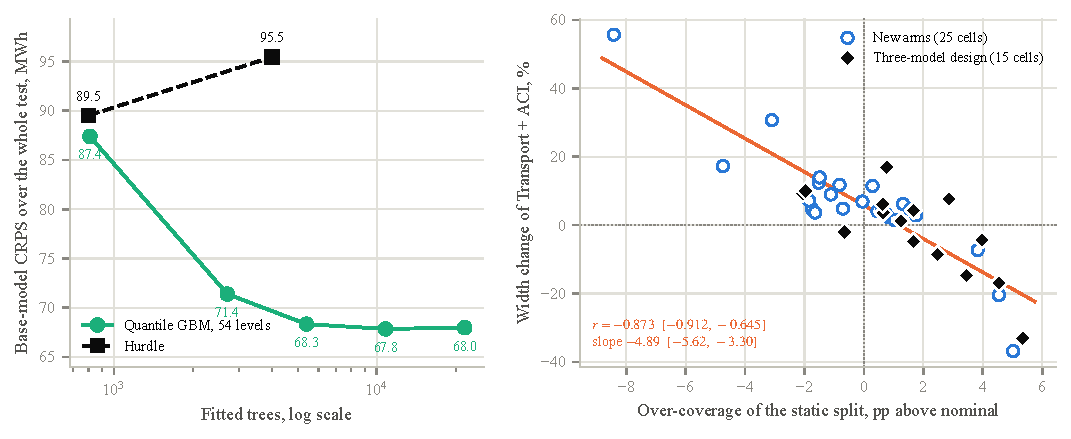
\includegraphics[width=\textwidth]{fig9_escalera_diagnostico.pdf}
\caption{Left: base-model CRPS over the whole test against the number of fitted trees, at a fixed 54-level quantile grid for the multi-quantile predictive. The hurdle is shown at its own budget and at five times it. Right: the diagnostic relationship over the forty cells, with the fifteen cells of the three-model design of Table~\ref{tab:diagnostico} marked separately, the fitted line over all forty, and its bootstrap interval. The new arms populate the region below nominal coverage, where the three-model design had no point.}
\label{fig:escalera}
\end{figure*}

\subsection{Which components earn their cost}
\label{sec:ablaciones}

The diagnostic above says the gain is attributable to the base model. The ablations say which parts of the calibration layer are doing anything at all. We ran five nested configurations, adding the pure static split and transport without adaptation to the three groups requested in review, so that each component can be isolated: static split, adaptive conformal inference alone, transport alone at a fixed level, transport plus adaptation without tail shrinkage, and the full scheme. Everything else is held fixed. Table~\ref{tab:ablaciones} reports the marginal contribution of each component to the interval score with a bootstrap interval over whole days, and Figure~\ref{fig:ablaciones} shows it window by window.

%% generated by flagship/revision/fase9_tablas_tex.py from resultados/
%% do not edit by hand
\begin{table*}[t]
\centering
\footnotesize
\caption{Marginal contribution of each component to the mean interval score, in MWh, with 95\% bootstrap intervals resampling whole days. Negative is an improvement. Runtime is the additional wall-clock cost of the component over the 638 test dates. Generated from \texttt{resultados/fase2/fase2\_aporte\_por\_componente.csv}.}
\label{tab:ablaciones}
\begin{tabular}{lccccccc}
\toprule
Component & \multicolumn{2}{c}{Transition window} & \multicolumn{2}{c}{Whole test} & Significant & Runtime (s) \\
\cmidrule(lr){2-3}\cmidrule(lr){4-5}
 & $\Delta\mathrm{IS}$ & 95\% CI & $\Delta\mathrm{IS}$ & 95\% CI & (whole test) & \\
\midrule
Online adaptation (ACI over static split) & $-297.9$ & $[-348, -251]$ & $-95.9$ & $[-118, -70]$ & yes & $+0.21$ \\
Transport alone (over static split) & $-282.9$ & $[-323, -245]$ & $-94.2$ & $[-111, -77]$ & yes & $+7.75$ \\
Transport added on top of ACI & $+12.0$ & $[-11, +36]$ & $+68.6$ & $[+41, +100]$ & yes & $+0.42$ \\
Tail shrinkage added on top of transport & $-0.6$ & $[-2, +0]$ & $-6.4$ & $[-10, -3]$ & yes & $+6.16$ \\
Full pipeline (over static split) & $-286.5$ & $[-351, -227]$ & $-32.3$ & $[-70, +9]$ & no & $+6.79$ \\
\bottomrule
\end{tabular}
\end{table*}


\begin{figure*}[t]
\centering
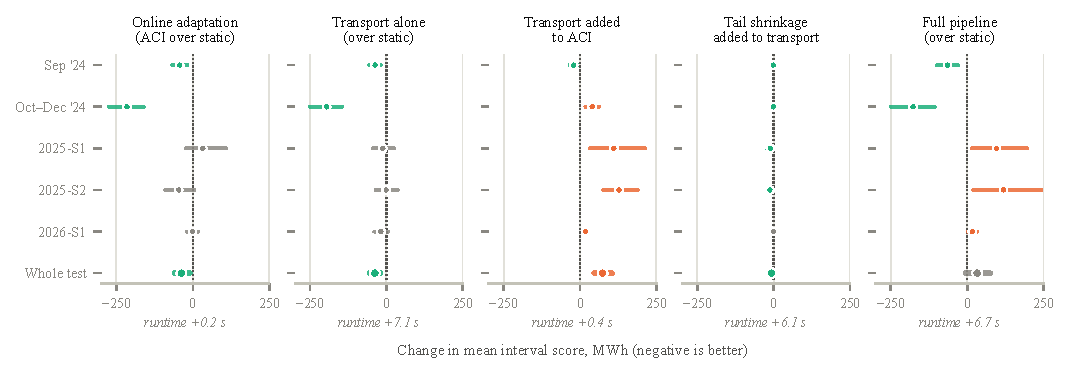
\includegraphics[width=\textwidth]{fig8_ablations.pdf}
\caption{Marginal contribution of each component of the adaptive scheme to the mean interval score, by window, with 95\% bootstrap intervals resampling whole days. Green marks a significant improvement, orange a significant deterioration, grey an interval containing zero. Runtime is the additional wall-clock cost of each component.}
\label{fig:ablaciones}
\end{figure*}

Three findings follow, and only the first is favourable.

Online adaptation earns its cost. Adding it to the static split improves the interval score by 297.9~MWh in the transition window, with a bootstrap interval of $[-348,-251]$, and by 95.9~MWh over the whole test, at a runtime cost of two tenths of a second.

Score transport does not, once adaptation is present. On top of the adaptive update it \emph{worsens} the interval score by 68.6~MWh over the whole test, with an interval of $[+41,+100]$ that excludes zero, and it worsens it in four of the five windows individually, significantly in three. Transport without adaptation does improve on the static split, by an amount statistically indistinguishable from what adaptation alone achieves, at thirty-seven times the runtime. The two components are substitutes rather than complements, and the cheaper one is at least as good.

The tail shrinkage does not pay for itself. Its effect on the whole test is $-6.4$~MWh with a bootstrap interval of $[-10,-3]$, which excludes zero but amounts to eight tenths of one per cent of an interval score of about 810, and it accounts for 6.16 of the 6.79 seconds the full pipeline costs, that is ninety-one per cent of the computational budget of the method.

Taken together the full pipeline improves on the static split by 286.5~MWh in the transition window and shows no demonstrable loss in any semester: in 2025-S1 and 2025-S2 the differences, $+58.8$ and $+14.3$~MWh, have intervals that contain zero, and in 2026-S1 it improves by 14.7~MWh with an interval that excludes zero. Over the whole test it nets $-32.3$~MWh with an interval of $[-70,+9]$ that contains zero: the complete method is not distinguishable from the static split it replaces, and we do not read that as a positive result for it.

\subsection{Metrics, infinite intervals and probabilistic benchmarks}
\label{sec:metricas}

Table~\ref{tab:benchmarks} evaluates every method on the whole test period under the full metric set, alongside four probabilistic benchmarks that the submitted version did not include: a per-plant empirical quantile over a trailing year, a per-plant rolling historical distribution over 60 days, a one-sided conformalized quantile regression~\cite{romano2019} on the multi-quantile predictive, and a per-plant zero-inflated lognormal fitted without covariates. All four respect the same nominal level, the same embargo and the same evaluation rows.

%% generated by flagship/revision/fase9_tablas_tex.py from resultados/
%% do not edit by hand
\begin{table*}[t]
\centering
\footnotesize
\caption{All methods on the whole test period, September 2024 to May 2026. Coverage in percent with date-clustered standard error, mean width in MWh over finite intervals, fraction of infinite intervals, interval score restricted to finite intervals, unrestricted interval score, and the bootstrap difference in interval score against the static split resampling whole days. The unrestricted score is the verdict: it is infinite for any method producing even one infinite limit. Generated from \texttt{resultados/fase4/}.}
\label{tab:benchmarks}
\begin{tabular}{lcccccc}
\toprule
Method & Coverage (se) & Width & \% inf. & $\mathrm{IS}$ finite & $\mathrm{IS}$ all & $\Delta\mathrm{IS}$ vs static [95\% CI] \\
\midrule
\multicolumn{7}{l}{\emph{Probabilistic benchmarks (new in this revision)}} \\
\quad B2 rolling historical distribution, 60 days, per plant & 86.5\,(0.51) & 282 & 0.0 & 433 & 433 & $-396$ $[-424, -368]$ \\
\quad B3 one-sided conformalized quantile regression (GBM) & 89.8\,(0.38) & 276 & 0.0 & 438 & 438 & $-391$ $[-419, -363]$ \\
\quad B1 empirical quantile, 365-day window, per plant & 87.2\,(0.51) & 317 & 0.0 & 486 & 486 & $-342$ $[-369, -314]$ \\
\quad B4 zero-inflated lognormal, per plant & 82.4\,(0.41) & 338 & 0.0 & 639 & 639 & $-192$ $[-217, -166]$ \\
\addlinespace
\multicolumn{7}{l}{\emph{Configuration selected by rolling origin}} \\
\quad Transport+ACI ($\gamma{=}0.005$, 120-day window) & 90.0\,(0.45) & 564 & 0.0 & 761 & 761 & $-65$ $[-83, -48]$ \\
\quad ACI ($\gamma{=}0.005$) & 90.9\,(0.41) & 590 & 0.0 & 763 & 763 & $-63$ $[-69, -57]$ \\
\addlinespace
\multicolumn{7}{l}{\emph{Methods of the submitted version}} \\
\quad Sliding window 60d & 89.9\,(0.44) & 531 & 0.0 & 734 & 734 & $-93$ $[-110, -76]$ \\
\quad ACI ($\gamma{=}0.02$) & 90.2\,(0.43) & 551 & 0.0 & 743 & 743 & $-83$ $[-98, -68]$ \\
\quad ACI ($\gamma{=}0.05$) & 90.1\,(0.43) & 544 & 4.2 & 753 & $\infty$ & $-96$ $[-118, -70]$ \\
\quad Transport+ACI ($\gamma{=}0.05$) & 90.1\,(0.43) & 596 & 5.9 & 813 & $\infty$ & $-32$ $[-70, +9]$ \\
\quad Static split (PIT) & 92.5\,(0.37) & 678 & 0.0 & 826 & 826 & -- \\
\quad Transport+ACI ($\gamma{=}0.02$) & 90.1\,(0.44) & 663 & 0.5 & 871 & $\infty$ & $+41$ $[-22, +116]$ \\
\bottomrule
\end{tabular}

\vspace{3pt}
\parbox{\linewidth}{\footnotesize Note: the last two columns are computed on different row sets, and in the three configurations that produce infinite limits the difference column is therefore not the subtraction of the finite-interval column. The $\mathrm{IS}$ finite column averages over the rows on which \emph{that} method returns a finite limit, so each row of the table uses a different denominator. The $\Delta\mathrm{IS}$ column is a paired comparison and is computed only on rows where \emph{both} the method and the static split are finite, which is the correct basis for a difference but discards up to 5.9\% of the rows; the fraction discarded is the infinite-interval fraction of the method, since the static split is finite throughout. For the methods with no infinite limits the two conventions coincide and the columns do subtract.}
\end{table*}


The benchmarks change the picture. All four attain a better interval score than every method built on the hurdle, and each differs from the static split by a day-block bootstrap interval that excludes zero. Three of them buy that score with coverage, and should be read accordingly: the rolling 60-day distribution reaches an interval score of 433 at 86.5\% coverage, the trailing-year quantile 486 at 87.2\% and the zero-inflated lognormal 639 at 82.4\%, all several points below nominal, so an operator who needs the stated level cannot use them. The conformalized quantile regression is the exception and is the most informative row of the table. It attains 89.8\% coverage, within half a point of nominal, with a mean width of 276~MWh and an interval score of 438, against 596~MWh and 813 for the full pipeline of the submitted version. A standard construction from 2019, applied to a better base predictive, dominates the method this paper proposed.

The treatment of infinite intervals matters and is now explicit. Three configurations of the submitted version produce infinite limits, up to 5.9 per cent of the test period, and under the width-over-finite-intervals convention they appear sharper than they are. The unrestricted interval score reports them as infinite, which is the correct verdict for a method that returns uninformative intervals.

The cause is structural rather than incidental: the adaptive update is allowed to drive $\alpha_t$ to zero or below, at which point the required order statistic does not exist and the conformal quantile is $+\infty$. Bounding the update from below removes the problem entirely. Table~\ref{tab:cota} shows the effect of $\alpha_{\min}\in\{0.005,0.01,0.02\}$. At $\alpha_{\min}=0.005$ the fraction of infinite intervals falls to zero in all five windows and all four adaptive configurations, at a cost of at most half a point of marginal coverage, and the unrestricted interval score becomes finite and therefore comparable. We recommend the bound as a default. It is worth noting what it does not fix: with infinities removed and the score made comparable, the transported variants remain worse than pure adaptation, which is the finding of Section~\ref{sec:ablaciones} rather than an artefact of the infinities.

%% generated by flagship/revision/fase9_tablas_tex.py from resultados/
%% do not edit by hand
\begin{table*}[t]
\centering
\footnotesize
\caption{Effect of bounding the online update of $\alpha$ from below, whole test period. A bound of $\alpha_{\min}=0.005$ removes infinite intervals entirely at negligible cost in coverage, and makes the unrestricted interval score finite and therefore comparable across methods. Generated from \texttt{resultados/fase4/fase4\_cota\_alpha.csv}.}
\label{tab:cota}
\begin{tabular}{lccccc}
\toprule
Bound on $\alpha_t$ & Coverage (se) & Width & \% infinite & $\mathrm{IS}$ finite & $\mathrm{IS}$ all \\
\midrule
\multicolumn{6}{l}{\emph{ACI ($\gamma{=}0.05$)}} \\
\quad unbounded (submitted version) & 90.1\,(0.43) & 544 & 4.2 & 753 & $\infty$ \\
\quad $\alpha_{\min}=0.005$ & 89.8\,(0.43) & 550 & 0.0 & 753 & 753 \\
\quad $\alpha_{\min}=0.01$ & 89.8\,(0.43) & 536 & 0.0 & 739 & 739 \\
\quad $\alpha_{\min}=0.02$ & 89.7\,(0.43) & 525 & 0.0 & 729 & 729 \\
\addlinespace
\multicolumn{6}{l}{\emph{Transport+ACI ($\gamma{=}0.05$)}} \\
\quad unbounded (submitted version) & 90.1\,(0.43) & 596 & 5.9 & 813 & $\infty$ \\
\quad $\alpha_{\min}=0.005$ & 89.6\,(0.43) & 641 & 0.0 & 850 & 850 \\
\quad $\alpha_{\min}=0.01$ & 89.6\,(0.43) & 598 & 0.0 & 807 & 807 \\
\quad $\alpha_{\min}=0.02$ & 89.5\,(0.43) & 559 & 0.0 & 770 & 770 \\
\bottomrule
\end{tabular}
\end{table*}


\subsection{Panel dependence and conditional coverage}
\label{sec:panel}

Clustered standard errors quantify the uncertainty that daily dependence induces in a reported coverage figure. They do not restore exchangeability, and the finite-sample guarantee of the split rests on exchangeability rather than on the width of a confidence interval. The distinction matters here because the dependence is severe: as reported in Section~\ref{sec:guarantees}, the intraclass correlation of the calibration score by date is 0.238, giving a design effect of 26.7 and an effective calibration sample of about 1{,}000 rows rather than 26{,}552.

We tested three families of remedy, and report what each one actually buys. Table~\ref{tab:panel} gives marginal performance together with the worst absolute deviation from nominal on each conditioning axis, which is the operative measure of conditional coverage.

%% generado por flagship/revision/fase9_tablas_tex.py
%% NO EDITAR A MANO: se regenera desde resultados/
\begin{table*}[t]
\centering
\footnotesize
\caption{Calibration schemes designed to address panel dependence, whole test period. The last four columns give the worst absolute deviation from the 90\% nominal level over the groups of each axis, in percentage points, which is the measure of conditional coverage; smaller is better. Generated from \texttt{resultados/fase5/}.}
\label{tab:panel}
\begin{tabular}{lcccrrrr}
\toprule
 & \multicolumn{3}{c}{Marginal} & \multicolumn{4}{c}{Worst deviation from nominal (pp)} \\
\cmidrule(lr){2-4}\cmidrule(lr){5-8}
Scheme & Coverage (se) & Width & $\mathrm{IS}$ & Technology & Size & Region & High-curt. \\
\midrule
Pooled split (submitted version) & 92.5\,(0.37) & 678 & 973 & 2.5 & 3.6 & 4.8 & 2.9 \\
Block conformal, one plant per date & 92.7\,(0.36) & 697 & 983 & 2.8 & 3.9 & 5.1 & 3.1 \\
Mondrian by technology & 92.3\,(0.37) & 651 & 967 & 4.1 & 3.7 & 5.1 & 2.7 \\
Mondrian by region & 92.1\,(0.38) & 596 & 933 & 4.0 & 3.7 & 7.2 & 2.5 \\
Mondrian by capacity tercile & 92.5\,(0.37) & 674 & 971 & 2.6 & 3.9 & 4.8 & 2.9 \\
Plant-level conformal & 92.5\,(0.39) & 636 & 909 & 4.1 & 3.0 & 7.2 & 2.8 \\
ACI ($\gamma{=}0.02$), for reference & 90.2\,(0.43) & 551 & 936 & 0.3 & 1.5 & 4.7 & 1.7 \\
Transport+ACI ($\gamma{=}0.05$), for reference & 90.1\,(0.43) & 593 & 1028 & 0.3 & 1.6 & 4.8 & 3.3 \\
\bottomrule
\end{tabular}
\end{table*}


\emph{Block conformal.} Subsampling one plant per date makes the calibration scores approximately independent at the cost of reducing them from 26{,}552 to 244. Averaged over 200 replicates with a fixed seed, the conformal quantile moves from 0.9242 to 0.9263, a difference of two thousandths of a PIT unit, while the replicate standard deviation of that quantile is 0.0112. The point estimate is therefore close to unbiased; what the pooled construction misstates is not the level but the precision, since the guarantee is nominally stated at a sample size twenty-seven times larger than the effective one. Marginal performance is essentially unchanged and conditional coverage is marginally worse, so this is a correction to the interpretation rather than an improvement to the method.

\emph{Group conformal.} Mondrian calibration with a separate conformal quantile per group restores group-conditional coverage by construction only if the group quantiles are well estimated. By technology and by capacity tercile the effect is small. By region it is harmful: the worst regional deviation rises from 4.8 to 7.2 percentage points, because several regions contribute too few calibration days for a stable quantile and the resulting estimates are noisy. Plant-level calibration, the finest partition, has the same problem in a stronger form and the same 7.2-point worst regional deviation, although it and Mondrian by region have the two best marginal interval scores of the group. This is a negative result worth recording: partitioning the calibration set is not a free way to buy conditional validity when the partition is fine relative to the effective sample size.

\emph{The adaptive schemes.} The best conditional coverage in the table belongs to plain adaptive conformal inference, with a worst deviation of 4.7 percentage points, better than every Mondrian variant. That is a point in favour of online adaptation, and it is consistent with the ablation result: adaptation is the component that works.

One conditional result deserves emphasis because it runs against the interest of the method. On high-curtailment days, defined by the calibration-window ninetieth percentile of system-level daily curtailment and covering 254 of the 638 test days, the static split covers at 91.9 per cent while Transport+ACI covers at 86.7 per cent. The economically important days are exactly where the adaptive scheme under-covers most, and a portfolio owner sizing an exposure on the largest days would be worse served by it than by the static split. Adaptive conformal inference sits between the two at 88.3 per cent.

\subsection{Sensitivity to the window boundary, the change-point dates and the calibration hyperparameters}
\label{sec:frontera}

The transition window is defined by a measurable criterion, but the criterion still has to be applied to some boundary, and one might ask whether the results are an artefact of that choice. Table~\ref{tab:frontera} re-evaluates the three representative methods on five alternative definitions of the window besides the one used, ranging from two months to seven. The Wasserstein-1 divergence from the calibration distribution varies from 0.99 to 1.34 across them, and the ordering of the three methods by coverage is the same in every case: the static split over-covers by 4.0 to 5.3 points, adaptive conformal inference sits between, and the transported variant covers least. By the interval score over finite intervals the static split is the worst of the three in all six; the transported variant returns infinite limits in three of them, 5.5 to 8.1 per cent, where its unrestricted score is infinite. The apparent gain of the transported variant follows how far the static split over-covers in each window (Pearson $r=-0.844$ across the six), which is the same relationship established in Section~\ref{sec:agnostic}, here traced in the boundary rather than across base models.

%% generated by flagship/revision/fase9_tablas_tex.py from resultados/
%% do not edit by hand
\begin{table*}[t]
\centering
\footnotesize
\caption{Sensitivity to alternative definitions of the transition window, hurdle base model. $W_1$ is the Wasserstein-1 distance between the positive log-magnitudes of the window and those of the calibration set. Generated from \texttt{resultados/fase6/fase6\_sensibilidad\_frontera.csv}.}
\label{tab:frontera}
\begin{tabular}{lccc}
\toprule
Method & Coverage (se) & Width & Interval score \\
\midrule
\multicolumn{4}{l}{\emph{Oct--Dec 2024 (the one used)}, $W_1 = 1.253$} \\
\quad Static split & 95.3\,(0.45) & 1203 & 1588 \\
\quad ACI ($\gamma{=}0.02$) & 93.5\,(0.55) & 915 & 1401 \\
\quad Transport+ACI ($\gamma{=}0.05$) & 90.9\,(0.81) & 806 & 1409 \\
\addlinespace
\multicolumn{4}{l}{\emph{Sep--Dec 2024}, $W_1 = 1.179$} \\
\quad Static split & 94.9\,(0.43) & 1105 & 1452 \\
\quad ACI ($\gamma{=}0.02$) & 93.4\,(0.49) & 877 & 1305 \\
\quad Transport+ACI ($\gamma{=}0.05$) & 91.1\,(0.67) & 776 & 1302 \\
\addlinespace
\multicolumn{4}{l}{\emph{Nov 2024--Jan 2025}, $W_1 = 1.109$} \\
\quad Static split & 94.8\,(0.79) & 1105 & 1406 \\
\quad ACI ($\gamma{=}0.02$) & 91.2\,(1.17) & 788 & 1250 \\
\quad Transport+ACI ($\gamma{=}0.05$) & 88.6\,(1.43) & 795 & 1373 \\
\addlinespace
\multicolumn{4}{l}{\emph{Oct 2024--Feb 2025}, $W_1 = 1.002$} \\
\quad Static split & 94.5\,(0.57) & 1000 & 1327 \\
\quad ACI ($\gamma{=}0.02$) & 91.2\,(0.83) & 732 & 1197 \\
\quad Transport+ACI ($\gamma{=}0.05$) & 89.5\,(1.01) & 791 & 1390 \\
\addlinespace
\multicolumn{4}{l}{\emph{Oct--Nov 2024}, $W_1 = 1.342$} \\
\quad Static split & 94.0\,(0.58) & 1108 & 1637 \\
\quad ACI ($\gamma{=}0.02$) & 92.4\,(0.73) & 896 & 1542 \\
\quad Transport+ACI ($\gamma{=}0.05$) & 89.9\,(1.08) & 842 & 1606 \\
\addlinespace
\multicolumn{4}{l}{\emph{Sep 2024--Mar 2025}, $W_1 = 0.992$} \\
\quad Static split & 94.3\,(0.5) & 968 & 1279 \\
\quad ACI ($\gamma{=}0.02$) & 91.5\,(0.72) & 736 & 1166 \\
\quad Transport+ACI ($\gamma{=}0.05$) & 89.9\,(0.87) & 772 & 1316 \\
\bottomrule
\end{tabular}
\end{table*}


The chronology itself is likewise insensitive to the analyst's choices, as reported in Section~\ref{sec:regime}: across 180 detection configurations, none returns a break in 2025 and none returns one in October 2024. The two dates that do appear, May 2023 and January 2024, are returned by both algorithms under the default penalty and are the two most frequent across the whole sensitivity grid.

\paragraph{Calibration hyperparameters} The selection of Section~\ref{sec:seleccion} used only the inner validation set and was closed before the test set was touched. Table~\ref{tab:sens_hiper} reports the full $6\times5$ grid on the test set, as a display, never as a criterion. For the transported variant coverage is flat in $\gamma$ and in the window, between 89.9 and 90.1 per cent over all thirty configurations, and what varies is the fraction of infinite intervals: none at $\gamma\le 0.01$, and between 21.9 and 23.0 per cent at $\gamma=0.20$.

%% generated by flagship/revision/fase9_tablas_tex.py from resultados/
%% do not edit by hand
\begin{table*}[t]
\centering
\footnotesize
\caption{Sensitivity of the adaptive schemes to the step $\gamma$ and to the length of the recent window, whole test period, September 2024 to May 2026. This table is a display produced after the selection of Section~\ref{sec:seleccion} was closed, never a criterion: the selection used only the inner validation set. Pure ACI has no window. Bold marks the configuration selected by rolling origin; the 60-day cells at $\gamma=0.02$ and $0.05$ are the configurations of the submitted version and coincide with Table~\ref{tab:benchmarks}. $^\dagger$The configuration produces infinite limits, so its unrestricted interval score is infinite. Generated from \texttt{resultados/fase3/fase3\_sensibilidad\_test.csv}.}
\label{tab:sens_hiper}
\begin{tabular}{lcccccc}
\toprule
 & ACI & \multicolumn{5}{c}{Transport+ACI, recent window (days)} \\
\cmidrule(lr){3-7}
$\gamma$ & & 30 & 45 & 60 & 90 & 120 \\
\midrule
\multicolumn{7}{l}{\emph{Coverage (\%)}} \\
\quad 0.005 & \textbf{90.9} & 89.9 & 90.0 & 90.0 & 90.0 & \textbf{90.0} \\
\quad 0.01 & 90.5 & 90.0 & 90.0 & 90.0 & 90.0 & 90.0 \\
\quad 0.02 & 90.2 & 90.0 & 90.1 & 90.1 & 90.0 & 90.0 \\
\quad 0.05 & 90.1 & 90.1 & 90.1 & 90.1 & 90.0 & 90.0 \\
\quad 0.10 & 90.1 & 90.0 & 90.0 & 90.0 & 90.0 & 90.0 \\
\quad 0.20 & 90.0 & 89.9 & 90.0 & 90.0 & 90.0 & 90.0 \\
\addlinespace
\multicolumn{7}{l}{\emph{Infinite intervals (\%)}} \\
\quad 0.005 & \textbf{0.0} & 0.0 & 0.0 & 0.0 & 0.0 & \textbf{0.0} \\
\quad 0.01 & 0.0 & 0.0 & 0.0 & 0.0 & 0.0 & 0.0 \\
\quad 0.02 & 0.0 & 0.0 & 0.3 & 0.5 & 0.6 & 1.1 \\
\quad 0.05 & 4.2 & 5.3 & 6.4 & 5.9 & 5.2 & 4.4 \\
\quad 0.10 & 1.6 & 6.2 & 4.2 & 4.4 & 3.6 & 4.3 \\
\quad 0.20 & 15.1 & 22.5 & 23.0 & 21.9 & 22.4 & 22.9 \\
\addlinespace
\multicolumn{7}{l}{\emph{Interval score over finite intervals (MWh)}} \\
\quad 0.005 & \textbf{763} & 775 & 759 & 753 & 756 & \textbf{761} \\
\quad 0.01 & 748 & 803 & 789 & 776 & 769 & 770 \\
\quad 0.02 & 743 & 898 & 905$^\dagger$ & 871$^\dagger$ & 846$^\dagger$ & 822$^\dagger$ \\
\quad 0.05 & 753$^\dagger$ & 826$^\dagger$ & 806$^\dagger$ & 813$^\dagger$ & 831$^\dagger$ & 895$^\dagger$ \\
\quad 0.10 & 784$^\dagger$ & 893$^\dagger$ & 804$^\dagger$ & 821$^\dagger$ & 817$^\dagger$ & 784$^\dagger$ \\
\quad 0.20 & 936$^\dagger$ & 872$^\dagger$ & 877$^\dagger$ & 769$^\dagger$ & 774$^\dagger$ & 769$^\dagger$ \\
\bottomrule
\end{tabular}
\end{table*}


%==================================================================
\section{Discussion}
\label{sec:discussion}

\subsection{What the diagnostic means for practice}

The central empirical result of this paper is negative, and it is worth stating what it does and does not license.

It does not say that adaptive conformal calibration is useless. Online adaptation is the one component that improves the interval score reliably in our ablations, it costs almost nothing to run, and it delivers the best conditional coverage of any scheme we tested. It does say that the headline gain of a calibration layer, measured as width recovered against a static split, is not a measurement of how much distribution shift the layer absorbed. On these data it is a measurement of how over-dispersed the base predictive was, and the relationship between the two is close enough to linear to be used as a diagnostic: a large apparent gain should prompt an examination of the base model before it is reported as a property of the calibration method.

The practical ordering that follows is the reverse of the one the submitted version implied. Fixing the base predictive dominates fixing the calibration layer. Replacing a constant-dispersion lognormal hurdle by a multi-quantile predictive fitted under the same protocol halves the interval width at the same coverage and improves the CRPS by a fifth to a third in every window, at a fitted budget of the order of five thousand trees against the hurdle's eight hundred, a budget the hurdle cannot use (Section~\ref{sec:escalera}), whereas the entire adaptive apparatus, run on the worse base model, recovers less and costs more. Once the base model is adequate, the simplest available calibration layer is competitive: a one-sided conformalized quantile regression on the multi-quantile predictive attains 89.8 per cent coverage at 276~MWh.

There is a methodological point here that generalises beyond curtailment. A calibration layer evaluated against a single base model cannot distinguish between correcting a shift and correcting the model. The experiment that separates them is cheap, since a well-designed layer touches the base model only through a CDF and its inverse, and we would argue it should be standard in this literature. Our own construction did not survive it.

\subsection{Where the operational value actually lies}

For plant-level curtailment at a seven-day horizon, and within the information set available from public data, effort is better spent on reliable uncertainty quantification than on chasing point accuracy, which a calendar baseline already delivers. That conclusion survives the revision. What changes is the recommendation about how to obtain the uncertainty: through a flexible, well-calibrated predictive distribution and a simple conformal wrapper, rather than through an elaborate adaptive layer over a rigid parametric one.

Two operational details from Section~\ref{sec:results} are worth carrying forward. Bounding the online update from below is a free improvement: at $\alpha_{\min}=0.005$ it removes infinite prediction limits entirely, at a coverage cost of at most half a point, and it should be the default in any deployment where an uninformative interval is worse than a slightly wrong one. And conditional reliability on the largest days is the property a portfolio owner should check first, because it is where the schemes differ most and where the money is: on high-curtailment days the adaptive scheme under-covers by more than three points relative to the static split.

\subsection{The change in the record, and what we do not claim about it}

The distributional change documented in Section~\ref{sec:regime} is real, is a ramp of roughly eighteen months between mid-2023 and late 2024, and is essentially complete before 2025 begins. On its causes we are deliberately agnostic, and the dataset released here cannot settle the question, because it records curtailment and not the assets or the network states that absorb it. Several mechanisms operate over the same months and cannot be separated with these data: the growth of solar capacity behind a saturated north-to-south corridor, reinforcements of that corridor, changes in northern mining demand, the entry of battery storage, and the mechanical saturation of curtailment itself once the corridor is full throughout the solar window. The literature discussed in Section~\ref{sec:related} makes clear how much would be needed to identify any of them: Mohamad et al.~\cite{mohamad2021} show that the effect of storage on curtailment depends on where it sits relative to the binding constraint, and Denholm and Mai~\cite{denholm2019} show that it depends on duration as much as on power. We have neither the locational network model nor the charge-discharge records that such an analysis requires.

A second and distinct phenomenon appears at the turn of 2024 to 2025: a break in the rate of growth. The year-over-year growth of the monthly mean log-magnitude falls to $+0.09$ per year for northern solar from January 2025 and to $+0.01$ at system level from December 2024, while the northern solar fleet keeps expanding by 8 per cent through 2025 and curtailment per installed MW in those regions falls by 15 per cent in the fourth quarter. Storage entry is one candidate for that flattening and is quantitatively of the right order, but the supporting energy balance is an upper bound that holds only under assumptions of one full daily cycle, unit efficiency and every charged megawatt-hour having otherwise been curtailed; the same exercise repeated for January to May 2026 does not reproduce it. We record storage as one bounded hypothesis among several and make no causal claim. A registry of storage systems with their commercial operation dates is provided in the supplementary material so that the hypothesis can be tested independently by anyone with the network and dispatch data we lack.

It is worth noting that the calibration layer responds to only one of these two kinds of change. A displacement of the level of the predictive law, such as the ramp of 2023 and 2024, appears as a displacement of the score distribution and is what the transport map and the online update are built to absorb. A break in the rate of growth is not, and none of the methods evaluated here detects it. That does not damage their coverage, because a trend that flattens leaves no displacement to correct, but it matters for interpretation: reliability under shifts of level carries no guarantee under changes of trend, and the two are not distinguishable from coverage alone.

\subsection{The mid-2025 excursion}

The coverage dip visible in Figure~\ref{fig:rolling} can be given a date and a signature. It is concentrated in June 2025, the largest deseasonalised monthly anomaly of the entire post-calibration record: the monthly mean log-magnitude for northern solar stands well above the deseasonalised level of the calibration window, and the Wasserstein-1 distance between May to July 2025 and August to December 2025 is 1.334, larger than the 1.147 of the transition contrast itself. Its signature is the reverse of the 2024 window: magnitudes rise while the occurrence probability falls, whereas in October to December 2024 the two rose together. It appears in solar and in wind separately and across four regions, which rules out a single plant or a residual erratum, and the operator's monthly report for that month records no storage system entering operation. A one-month excursion with an occurrence signature opposite to that of the main transition is the kind of event that a continuously adapting scheme absorbs only slowly and that a change-point trigger would catch, which is one of the directions we identify below.

\subsection{Open directions}

Three follow directly from the results. A change-point detector could trigger recalibration at the onset of a shift rather than adapting continuously, which would address the June 2025 excursion; the machinery used offline in Section~\ref{sec:regime} to date the breaks is a natural starting point for an online version. Localised conformal prediction in the sense of Guan~\cite{guan2022}, which weights the calibration set by proximity to the test point, is a more principled route to conditional validity than the Mondrian partitions that failed in Section~\ref{sec:panel}, and it does not suffer from the small-group problem that defeated them. And extending the evaluation to the multivariate setting, across plants that share a transmission corridor and whose curtailment is therefore jointly determined, is the natural next step for an operator who manages a portfolio rather than an asset.

%==================================================================
\section{Limitations}
\label{sec:limitations}

Both reviewers of the submitted version noted that its limitations were understated. They were, and the following are the ones we consider material.

\emph{The scope of the point-forecasting conclusion.} Section~\ref{sec:punto} compares five model classes on a twelve-feature set at a seven-day horizon under mean absolute error. It does not establish anything about point forecasting of curtailment in general, and in particular says nothing about models with access to network topology, dispatch schedules, weather forecasts or storage state of charge, nor about criteria that weight large-magnitude days more heavily.

\emph{Exchangeability fails, and the finite-sample guarantee is correspondingly weaker than it looks.} The static split's guarantee is marginal and requires exchangeability, which does not hold here either across the regime boundary or within a regime. The effective calibration sample is about 1{,}000 rows rather than 26{,}552 (Section~\ref{sec:guarantees}), so the nominal finite-sample statement is stated at a sample size the data do not supply. None of the block, group or plant-level schemes of Section~\ref{sec:panel} repairs this; the block scheme quantifies it, and the group schemes make conditional coverage worse.

\emph{The diagnostic rests on two model families and one dataset.} The relationship between over-coverage and width recovery is established over forty cells from eight predictives on one panel, but the eight are not eight model classes: three are variants of the hurdle family and five are budget variants of a single quantile family. The design therefore spans two functional forms, not eight. We regard it as a mechanism that generalises, since it follows from what a conformal quantile does, but we have not demonstrated that it holds in other systems or with other model families, and the specific coefficients should not be transported.

\emph{The separation of model form from fitted capacity rests on one panel and two model families.} Section~\ref{sec:escalera} settles, for this problem, a question that the comparison of Section~\ref{sec:agnostic} leaves open: the multi-quantile advantage is not available at the hurdle's own tree budget, the hurdle does not recover it when given five times that budget, and at comparable budgets the gap is about thirty per cent. What that licenses is a statement about these two families on this panel. It does not license a statement about quantile regression against two-part models in general, and we do not make one. Two features of the ladder bound it further. It varies budget only through the number of trees, holding depth, learning rate and the rest fixed, so it separates budget from form along one axis and not all of them. The ladder itself uses no early stopping, so the enlarged hurdle is free to overfit rather than to halt. We fitted an early-stopped hurdle separately, reported in Section~\ref{sec:escalera}: it selects 105 trees, an eighth of our base model's budget, and beats that base model by 5.7 per cent of CRPS. Our base model is therefore not the best hurdle available on this problem, and every level we report for it, and every difference computed from it, should be read with that discount: Table~\ref{tab:results}, the ablations of Table~\ref{tab:ablaciones}, the benchmark comparison of Table~\ref{tab:benchmarks}, the $\alpha$ bound of Table~\ref{tab:cota}, the panel-dependence schemes of Table~\ref{tab:panel}, the boundary sensitivity of Table~\ref{tab:frontera}, and Figures~\ref{fig:rolling}, \ref{fig:tradeoff} and \ref{fig:ablaciones}. None of those tables was re-run with the stopped hurdle, so we claim no direction for the discount there. The one comparison that was re-run is the point forecasting of Table~\ref{tab:mae}, which is deliberately not in that list, and there the discount runs the other way: the stopped fit is better by CRPS but worse by mean absolute error, enough to place it last (Section~\ref{sec:punto}). What does hold is the margin to the quantile form, which stays above twenty per cent over the whole test. A reader comparing model families on our numbers should compare against the stopped hurdle rather than against ours.

\emph{The multi-quantile predictive has its own boundaries.} It expresses nothing above its highest estimated quantile level, $\tau=0.999$, and requests beyond it return an infinite limit. In this evaluation no interval hit that boundary, but a more extreme test period could, and the failure mode is not hypothetical: an arm fitted on a nine-level grid, whose top level is $\tau=0.9$, returns an infinite limit for every test row under the static split, because the conformal quantile of 0.938 falls above the highest level the predictive expresses. That arm is excluded from Table~\ref{tab:escalera} and from the diagnostic of Section~\ref{sec:agnostic}; it is recorded here as a mechanical demonstration of where a quantile-grid predictive breaks. Its implied occurrence probability is also coarse, read off the quantile grid at 0.02 resolution, which is why its Brier score is worse than the hurdle's and why that comparison is reported as descriptive rather than as a verdict.

\emph{Differences of one to three points of coverage are within the date-clustered standard error} and we have avoided interpreting them. Where a difference matters to a conclusion we report a bootstrap interval over whole days and state whether it excludes zero.

\emph{The hyperparameter selection uses a short inner validation set.} Because base-model predictions begin in January 2024, the rolling-origin selection of Section~\ref{sec:seleccion} runs on four months of inner validation. That is enough to reject the aggressive settings, which produce infinite intervals in a third of validation cases, but it is a thin basis for fine distinctions among the gentler ones.

\emph{The causes of the distributional change are not identified and cannot be with this dataset.} We record storage as one bounded hypothesis among several for the trend break at the turn of 2024 to 2025, and we make no causal claim. The supplementary registry is offered so that others can test it with data we do not have.

\emph{The dataset records curtailment only.} It contains no network state, no dispatch decision, no price and no storage operation, so every mechanism discussed in Section~\ref{sec:discussion} is outside what it can adjudicate.

%==================================================================
\section{Conclusion}
\label{sec:conclusion}

We have presented an open, errata-corrected, plant-level dataset of renewable curtailment covering 53 continuous months and 300 plants, whose annual totals reconcile exactly with the system operator's published figures, and we have used it to evaluate conformal calibration under a documented distributional change.

The empirical findings are these. Within the models, features, horizon and metric tested, point forecasting adds little over a calendar baseline, so the operationally relevant problem is uncertainty quantification. A regime shift of the kind observed here inflates standard conformal intervals into over-covered, wider bands rather than breaking their coverage. A substantial share of what reads as regime change is the annual cycle and has to be separated from it before the shift can be sized. And the gain that an adaptive conformal layer appears to deliver against that shift is, on these data, a measurement of the base model's over-dispersion rather than of the shift: it does not replicate when the base predictive is replaced by a multi-quantile alternative fitted under the same protocol, it is linearly related to how much the static split over-covers, and its two most elaborate components, score transport and bootstrap tail shrinkage, do not survive ablation. A conformalized quantile regression on the better base model attains near-nominal coverage at less than half the width of the full pipeline.

Three guarantees should be kept apart when such results are reported, and we have kept them apart throughout. The static split provides finite-sample \emph{marginal} coverage under exchangeability, an assumption this panel violates both across the regime boundary and within it, with an effective calibration sample twenty-seven times smaller than the nominal one. The adaptive update provides long-run average coverage control without any distributional assumption, and nothing at finite time. Empirical coverage in a dependent panel is a third thing, is what we measure, and is what varies across technologies, plant sizes, regions and high-curtailment days in the ways reported here.

The dataset and the code that regenerates every table and figure are publicly available, and we hope both the resource and the negative result are useful to operators, asset owners and researchers working on the integration of variable renewable energy.

%==================================================================
\section*{CRediT authorship contribution statement}
\textbf{Pablo Reyes Cerda:} Conceptualization, Data curation, Software, Validation, Investigation, Writing -- original draft. \textbf{Kerven Cea Morales:} Methodology, Formal analysis, Validation, Writing -- review and editing.

\section*{Declaration of competing interest}
Pablo Reyes Cerda is the founder of Synapta SpA and of CurtailmentIQ, a commercial forecasting service that uses data sources related to those described in this article. Kerven Cea Morales declares no competing interest.

\section*{Declaration of generative AI in scientific writing}
During the preparation of this work the authors used an AI-based assistant to improve the readability and language of the manuscript. After using this tool, the authors reviewed and edited the content as needed and take full responsibility for the content of the article.

\section*{Data availability}
The dataset is openly available on Zenodo under a CC~BY~4.0 licence (DOI: 10.5281/zenodo.21198816, which resolves to the latest version of the deposit). The processing pipeline, the modelling code and the scripts that regenerate every table and figure in this article are available in the companion repository at \url{https://github.com/Pablosebastian-reyes/curtailmentiq-research}. The supplementary material accompanying this article contains a registry of the energy storage systems of the SEN with their commercial operation dates and sources, compiled from the public reports of the system operator, the Ministry of Energy and the National Energy Commission; it is offered so that the bounded hypothesis of Section~\ref{sec:discussion} can be tested independently, and it is not part of the released dataset.

%==================================================================
\appendix

\section{Inversion of the PIT limit}
\label{app:inversion}

Fix $x$ and write $p=p(x)$, $\mu=\mu(x)$. The mixture CDF is $F_x(y)=0$ for $y<0$, $F_x(0)=1-p$, and $F_x(y)=(1-p)+p\,\Phi\big((\log y-\mu)/\sigma\big)$ for $y>0$, which is continuous and strictly increasing on $(0,\infty)$ from $1-p$ to $1$. Given a level $\hat q\in[0,1]$ we seek the smallest $u\ge 0$ with $F_x(u)\ge \hat q$. If $\hat q\le 1-p$ the atom already reaches the level, so $u=0$. If $\hat q\ge 1$ no finite $u$ attains it and $u=+\infty$. For $1-p<\hat q<1$, strict monotonicity gives a unique solution of $(1-p)+p\,\Phi\big((\log u-\mu)/\sigma\big)=\hat q$, that is $\Phi\big((\log u-\mu)/\sigma\big)=(\hat q-(1-p))/p\in(0,1)$, hence $\log u=\mu+\sigma\,\Phi^{-1}\big((\hat q-(1-p))/p\big)$ and
\[
U(x)=\exp\!\Big(\mu+\sigma\,\Phi^{-1}\big(\tfrac{\hat q-(1-p)}{p}\big)\Big),
\]
which is~\eqref{eq:invert}. The two boundary cases are recovered as the limits of the clipped argument $(\hat q-(1-p))/p\to 0^+$ and $\to 1^-$, since $\Phi^{-1}(0^+)=-\infty$ gives $U=0$ and $\Phi^{-1}(1^-)=+\infty$ gives $U=+\infty$. \qed

For the multi-quantile predictive the same object is obtained without a closed form. Let $\tau_1<\dots<\tau_K$ be the estimated levels and $\hat q_{\tau_1}(x)\le\dots\le\hat q_{\tau_K}(x)$ the rearranged quantiles, and augment the grid with the node $(0,0)$. Then $F_x$ is the piecewise-linear interpolant of the augmented pairs, its atom is $F_x(0)=\max\{\tau_k:\hat q_{\tau_k}(x)=0\}$, and $F_x^{-1}(\hat q)$ is the piecewise-linear interpolant in the other direction, equal to $0$ for $\hat q\le F_x(0)$ and to $+\infty$ for $\hat q>\tau_K$.

\section{Coverage under score transport}
\label{app:coverage}

\emph{Static split.} If the calibration scores $s_1,\dots,s_n$ and the test score $s_{n+1}$ are exchangeable, then with $\hat q=s_{(k)}$, $k=\lceil(n+1)(1-\alpha)\rceil$, one has $\mathbb{P}(s_{n+1}\le\hat q)\ge k/(n+1)\ge 1-\alpha$, and since $F_x$ is monotone, $s_{n+1}\le\hat q$ if and only if $Y\le U(x)$; hence $\mathbb{P}(Y\le U(x))\ge 1-\alpha$. This is a \emph{marginal} statement, and it is exact only under exchangeability; the serial and cross-sectional dependence of the panel make it approximate. Section~\ref{sec:guarantees} quantifies how approximate: with an intraclass correlation by date of 0.238 and 108.8 plants per day, the effective $n$ is about 1{,}000 rather than 26{,}552, so the guarantee should be read at the smaller sample size.

\emph{Transported scores.} Let $P_{\mathrm{old}}$ and $P_{\mathrm{new}}$ be the laws of the score in the old and new regimes and $T=F_{\mathrm{new}}^{-1}\circ F_{\mathrm{old}}$ the monotone transport map. Under an \emph{oracle} map, $T(s)\sim P_{\mathrm{new}}$ for $s\sim P_{\mathrm{old}}$, so the transported calibration scores are exchangeable with the test score and the static guarantee transfers exactly. With an \emph{estimated} map $\hat T$ the transported scores are only approximately distributed as $P_{\mathrm{new}}$, and the coverage gap is bounded by the total-variation distance $d_{\mathrm{TV}}\big(\hat T_\# P_{\mathrm{old}},P_{\mathrm{new}}\big)$ through the weighted-exchangeability framework of Barber et al.~\cite{barber2023}. We do not rely on this bound in practice: because $\hat T$ is data-dependent and the gap is not directly controllable, we obtain validity operationally by feeding the transported scores into the adaptive update of Gibbs and Cand\`es~\cite{gibbs2021}, whose long-run coverage $\frac1T\sum_t\mathrm{err}_t\to\alpha$ holds for any sequence, so that the transport contributes sharpness and the online control contributes coverage. Section~\ref{sec:ablaciones} reports that on these data the sharpness contribution is negative once the online control is present.

\section{Hyperparameters, constants and seeds}
\label{app:hiper}

Table~\ref{tab:hiper} lists every constant of the pipeline. It is generated directly from the source code rather than transcribed, by a script that imports the modules and reads the constants and default arguments, so that it cannot drift from the implementation.

%% generated from the source code by flagship/revision/fase1_hiperparametros.py
%% do not edit by hand
\begingroup
\footnotesize
\setlength{\LTcapwidth}{\textwidth}
\begin{longtable}{p{0.30\textwidth}p{0.22\textwidth}p{0.40\textwidth}}
\caption{Complete hyperparameter specification. Generated from the source by \texttt{flagship/revision/fase1\_hiperparametros.py}; the companion CSV records where each value lives in the code.}
\label{tab:hiper} \\
\toprule
Item & Value & Detail \\
\midrule
\endfirsthead
\multicolumn{3}{l}{\emph{Table \ref{tab:hiper}, continued.}} \\
\toprule
Item & Value & Detail \\
\midrule
\endhead
\midrule
\multicolumn{3}{r}{\emph{continued on the next page}} \\
\endfoot
\bottomrule
\endlastfoot
\multicolumn{3}{l}{\emph{Base model}} \\
Forecast horizon & 7 days & direct forecast; every dynamic feature is a shift of at least H days \\
Last training target & 2023-12-31 & the model never sees the evaluation period \\
Trees / learning rate / depth & 400 / 0.05 / 6 & fixed a priori, never tuned against 2024-2026 \\
min\_child\_weight / subsample / colsample & 5 / 0.9 / 0.9 & as above \\
Number of features & 12 & mwh\_t, mwh\_lag1, mwh\_lag7, mwh\_lag14, ma7\_t, ma30\_t, occ\_t, dow\_target, doy\_target, log\_potencia\_mw, region, tecnologia \\
Dispersion of the hurdle & out of fold, KFold 5 & in-sample residuals of a boosted model understate the dispersion \\
Quantile grid of the multi-quantile GBM & 54 levels, from 0.005 to 0.999 & 0.02 to 0.98 in steps of 0.02, plus 0.005, 0.01, 0.99, 0.995 and 0.999; row-wise rearrangement against quantile crossing \\
\midrule
\multicolumn{3}{l}{\emph{Conformal layer}} \\
Nominal level & 1 - alpha = 0.90 & one-sided upper prediction limit [0, U] \\
Nonconformity score & s = F\_x(y) (PIT) & atom at y = 0 randomised, s = (1-p)U with U ~ Uniform(0,1) \\
Calibration window & 2024-01-01 to 2024-09-01 & 244 days, 26,552 rows \\
Horizon embargo & 7 days & every online window ends at t-7 and the feedback of alpha is delayed by 7 steps \\
Conformal quantile & order statistic k = ceil((n+1)(1-alpha\_t)) & q = +infinity if k > n, which is the origin of the infinite intervals \\
\midrule
\multicolumn{3}{l}{\emph{Transport}} \\
Length of the recent window & 60 days & the window ends at t minus the embargo, not at t \\
Refresh period of the map & 7 days & the map is recomputed every 7 days; between refreshes the pool is frozen \\
Minimum recent scores for a refresh & 100 & with fewer scores in the recent window the previous pool is kept \\
Rule for the empirical quantiles & equispaced grid of g levels on [0,1], g = min(100, max(20, m/2)) & m is the number of scores in the recent window; the second term prevents a grid finer than the data \\
Interpolation scheme & piecewise linear, twice & first s -> level on (q\_old, levels), then level -> q\_reg on (levels, q\_reg); this is the increasing rearrangement T = F\_new\^\{\}\{-1\} o F\_old \\
Bootstrap repetitions of the map & B = 150 & resampling of the recent window with replacement; the mean of the B replicates is the map (bagging) and their standard deviation per level is the band \\
Tail shrinkage function & lambda(u) = 1 / (1 + (sd\_boot(u)/tau)\^\{\}2) & q\_reg(u) = (1-lambda(u)) q\_old(u) + lambda(u) q\_new\_bag(u); lambda ~ 1 where the map is stable and ~ 0 where it is noisy, and lambda = 0 is the identity, that is the old quantile \\
Shrinkage strength & tau = 0.05 in PIT units & fixed regularisation scale, not tuned against the test set \\
Monotonisation & running maximum and clip to [0,1] & keeps the transported map a quantile function \\
\midrule
\multicolumn{3}{l}{\emph{ACI}} \\
Update & alpha\_\{t+1\} = alpha\_t + gamma (alpha - err\_t) & err\_t = 1\{Y\_t > U\_t\}, averaged over the plants of day t \\
gamma reported in the submitted version & 0.02 and 0.05 & kept in the tables for continuity \\
Bound on alpha\_t, submitted version & [-1, 2] & allows alpha\_t <= 0 and hence q = +infinity: the origin of the infinite intervals \\
Recommended bound on alpha\_t & alpha\_min = 0.005 & removes infinite intervals in all five windows at a cost of at most 0.5 points of coverage \\
Order of execution & map refresh, then quantile, then interval, then ACI & on date t: (i) if a refresh is due, the map is recomputed from the window ending at t-7 and the whole calibration pool is transported; (ii) the quantile is taken from the transported pool at the CURRENT alpha\_t, which does not yet include the error of t; (iii) the interval is emitted; (iv) the error of t enters the embargo queue and updates alpha only 7 steps later. The map never uses the alpha of ACI and ACI never uses the map: the only coupling is the pool \\
\midrule
\multicolumn{3}{l}{\emph{Hyperparameter selection}} \\
Grid for gamma & \{0.005, 0.01, 0.02, 0.05, 0.10, 0.20\} & the test set is not used in the selection \\
Grid for the recent window & \{30, 45, 60, 90, 120\} days & Transport+ACI only \\
Inner calibration pool & 2024-01-01 to 2024-05-01 & first part of the calibration window \\
Inner validation set & 2024-05-01 to 2024-09-01 & rolling origin with the same 7-day refresh and 7-day embargo as the test protocol \\
Selection criterion & mean one-sided interval score & +infinity if any interval is infinite, so such a configuration is disqualified by the criterion itself; the generator uses the seed of the PIT atom \\
gamma selected by rolling origin & 0.005 & lowest interval score on the inner validation set; no infinite intervals there \\
Window selected by rolling origin & 120 days & as above, for Transport+ACI \\
\midrule
\multicolumn{3}{l}{\emph{Evaluation}} \\
Primary metric & one-sided interval score IS = U + (2/alpha) max(y-U, 0) & proper, in MWh, and infinite if U is infinite \\
Standard error of coverage & clustered by date & averages the coverage of each day and takes the error across days \\
Bootstrap of the differences between methods & 2000 resamples of whole days & the resampled unit is the day, not the row; 95\% percentile interval \\
Samples for the CRPS & 300 per row & sampled CRPS, E|X-y| - 0.5 E|X-X'| \\
Change-point detection & PELT and binary segmentation, L2 cost, pen = sigma\^\{\}2 log n, min\_size = 3 & BIC penalty with k = 1; the sensitivity grid spans k in \{0.5, 1, 2, 3, 5\} and min\_size in \{2, 3, 4\} \\
\midrule
\multicolumn{3}{l}{\emph{Seeds}} \\
Training of the base models & 42 & deterministic XGBoost hist, n\_jobs = 4, KFold \\
PIT atom and map bootstrap & 20260720 & a single generator consumed in order: first the score, then gamma = 0.02 and then gamma = 0.05 \\
Sampling of the CRPS & 11 &  \\
Bootstrap of differences, blocks and permutations & 20260901 &  \\
\end{longtable}
\endgroup


\section{Reproducibility}
\label{app:repro}

Every table and figure is regenerated by a versioned script from the frozen dataset. The environment is python 3.12.3 with pandas 3.0.3, numpy 2.4.6, scikit-learn 1.9.0, xgboost 3.2.0, ruptures 1.1.10 and statsmodels 0.15.0. The seeds are 42 for base-model training, 20260720 for the randomisation of the PIT atom and the bootstrap of the transport map, 11 for the CRPS sampling and 20260901 for the day-block bootstrap and the permutation nulls. The order in which the conformal generator is consumed is fixed and documented, which is what allows the hurdle arm of the model-agnosticism experiment to reproduce Table~\ref{tab:results} bit for bit. The command sequence that regenerates the entire set of results, together with a log of every run, is in the companion repository.

The model-agnosticism experiment of Section~\ref{sec:agnostic} was reproduced independently from a clean clone of the repository, in an environment resolved from the specification file rather than copied, in which four of the five principal libraries resolved to versions other than the reference ones. The retrained multi-quantile base model matched the versioned one by SHA-256 checksum, and the regenerated tables matched the published ones cell by cell, the only difference being wall-clock timing columns. The dataset files, which are distributed through the archive rather than the repository, were verified against the checksums versioned here before use.

%==================================================================
\begin{thebibliography}{99}

\bibitem{oshaughnessy2020}
E.~O'Shaughnessy, J.~R.~Cruce, K.~Xu,
Too much of a good thing? Global trends in the curtailment of solar PV,
Solar Energy 208 (2020) 1068--1077.
doi:10.1016/j.solener.2020.08.075.

\bibitem{henriot2015}
A.~Henriot,
Economic curtailment of intermittent renewable energy sources,
Energy Economics 49 (2015) 370--379.
doi:10.1016/j.eneco.2015.03.002.

\bibitem{joos2018}
M.~Joos, I.~Staffell,
Short-term integration costs of variable renewable energy: wind curtailment and balancing in Britain and Germany,
Renewable and Sustainable Energy Reviews 86 (2018) 45--65.
doi:10.1016/j.rser.2018.01.009.

\bibitem{tang2018}
N.~Tang, Y.~Zhang, Y.~Niu, X.~Du,
Solar energy curtailment in China: status quo, reasons and solutions,
Renewable and Sustainable Energy Reviews 97 (2018) 509--528.
doi:10.1016/j.rser.2018.07.021.

\bibitem{schermeyer2018}
H.~Schermeyer, C.~Vergara, W.~Fichtner,
Renewable energy curtailment: a case study on today's and tomorrow's congestion management,
Energy Policy 112 (2018) 427--436.
doi:10.1016/j.enpol.2017.10.037.

\bibitem{nycander2020}
E.~Nycander, L.~S\"oder, J.~Olauson, R.~Eriksson,
Curtailment analysis for the Nordic power system considering transmission capacity, inertia limits and generation flexibility,
Renewable Energy 152 (2020) 942--960.
doi:10.1016/j.renene.2020.01.059.

\bibitem{yildiz2023}
B.~Yildiz, N.~Stringer, T.~Klymenko, M.~Syahman~Samhan, G.~Abramowitz, A.~Bruce, I.~MacGill, R.~Egan,
Real-world data analysis of distributed PV and battery energy storage system curtailment in low voltage networks,
Renewable and Sustainable Energy Reviews 186 (2023) 113696.
doi:10.1016/j.rser.2023.113696.

\bibitem{bunodiere2020}
A.~Bunodiere, H.~S.~Lee,
Renewable energy curtailment: prediction using a logic-based forecasting method and mitigation measures in Kyushu, Japan,
Energies 13 (18) (2020) 4703.
doi:10.3390/en13184703.

\bibitem{denholm2019}
P.~Denholm, T.~Mai,
Timescales of energy storage needed for reducing renewable energy curtailment,
Renewable Energy 130 (2019) 388--399.
doi:10.1016/j.renene.2018.06.079.

\bibitem{wang2019}
B.~Wang, M.~Zhou, B.~Xin, X.~Zhao, J.~Watada,
Analysis of operation cost and wind curtailment using multi-objective unit commitment with battery energy storage,
Energy 178 (2019) 101--114.
doi:10.1016/j.energy.2019.04.108.

\bibitem{rayit2021}
N.~S.~Rayit, J.~I.~Chowdhury, N.~Balta-Ozkan,
Techno-economic optimisation of battery storage for grid-level energy services using curtailed energy from wind,
Journal of Energy Storage 39 (2021) 102641.
doi:10.1016/j.est.2021.102641.

\bibitem{mohamad2021}
F.~Mohamad, J.~Teh, C.-M.~Lai,
Optimum allocation of battery energy storage systems for power grid enhanced with solar energy,
Energy 223 (2021) 120105.
doi:10.1016/j.energy.2021.120105.

\bibitem{vargas2015}
L.~S.~Vargas, G.~Bustos-Turu, F.~Larrain,
Wind power curtailment and energy storage in transmission congestion management considering power plants ramp rates,
IEEE Transactions on Power Systems 30 (5) (2015) 2498--2506.
doi:10.1109/TPWRS.2014.2362922.

\bibitem{fang2021}
X.~Fang, H.~Cui, E.~Du, F.~Li, C.~Kang,
Characteristics of locational uncertainty marginal price for correlated uncertainties of variable renewable generation and demands,
Applied Energy 282 (2021) 116064.
doi:10.1016/j.apenergy.2020.116064.

\bibitem{foss1983}
S.~D.~Foss, S.~H.~Lin, R.~A.~Fernandes,
Dynamic thermal line ratings part I: dynamic ampacity rating algorithm,
IEEE Transactions on Power Apparatus and Systems PAS-102 (6) (1983) 1858--1864.
doi:10.1109/TPAS.1983.317795.

\bibitem{teh2016}
J.~Teh, I.~Cotton,
Reliability impact of dynamic thermal rating system in wind power integrated network,
IEEE Transactions on Reliability 65 (2) (2016) 1081--1089.
doi:10.1109/TR.2015.2495173.

\bibitem{lai2022}
C.-M.~Lai, J.~Teh,
Comprehensive review of the dynamic thermal rating system for sustainable electrical power systems,
Energy Reports 8 (2022) 3263--3288.
doi:10.1016/j.egyr.2022.02.085.

\bibitem{glaum2023}
P.~Glaum, F.~Hofmann,
Leveraging the existing German transmission grid with dynamic line rating,
Applied Energy 343 (2023) 121199.
doi:10.1016/j.apenergy.2023.121199.

\bibitem{su2025}
Y.~Su, M.~Tan, J.~Teh,
Short-term transmission capacity prediction of hybrid renewable energy systems considering dynamic line rating based on data-driven model,
IEEE Transactions on Industry Applications (2025).
doi:10.1109/TIA.2025.3529824.

\bibitem{maximov2016}
S.~Maximov, V.~Venegas, J.~L.~Guardado, E.~L.~Moreno, R.~L\'opez,
Analysis of underground cable ampacity considering non-uniform soil temperature distributions,
Electric Power Systems Research 132 (2016) 22--29.
doi:10.1016/j.epsr.2015.11.005.

\bibitem{oclon2021}
P.~Ocło\'n,
The effect of soil thermal conductivity and cable ampacity on the thermal performance and material costs of underground transmission line,
Energy 231 (2021) 120803.
doi:10.1016/j.energy.2021.120803.

\bibitem{lei2021}
X.~Lei, Z.~Yang, J.~Yu, J.~Zhao, Q.~Gao, H.~Yu,
Data-driven optimal power flow: a physics-informed machine learning approach,
IEEE Transactions on Power Systems 36 (1) (2021) 346--354.
doi:10.1109/TPWRS.2020.3001919.

\bibitem{kruse2023}
J.~Kruse, E.~Cramer, B.~Sch\"afer, D.~Witthaut,
Physics-informed machine learning for power grid frequency modeling,
PRX Energy 2 (4) (2023) 043003.
doi:10.1103/PRXEnergy.2.043003.

\bibitem{kirchnerbossi2024}
N.~Kirchner-Bossi, G.~Kathari, F.~Port\'e-Agel,
A hybrid physics-based and data-driven model for intra-day and day-ahead wind power forecasting considering a drastically expanded predictor search space,
Applied Energy 367 (2024) 123375.
doi:10.1016/j.apenergy.2024.123375.

\bibitem{maciejowska2016}
K.~Maciejowska, J.~Nowotarski, R.~Weron,
Probabilistic forecasting of electricity spot prices using factor quantile regression averaging,
International Journal of Forecasting 32 (3) (2016) 957--965.
doi:10.1016/j.ijforecast.2014.12.004.

\bibitem{uniejewski2021}
B.~Uniejewski, R.~Weron,
Regularized quantile regression averaging for probabilistic electricity price forecasting,
Energy Economics 95 (2021) 105121.
doi:10.1016/j.eneco.2021.105121.

\bibitem{vandermeer2018}
D.~W.~van~der~Meer, J.~Munkhammar, J.~Wid\'en,
Probabilistic forecasting of solar power, electricity consumption and net load: investigating the effect of seasons, aggregation and penetration on prediction intervals,
Solar Energy 171 (2018) 397--413.
doi:10.1016/j.solener.2018.06.103.

\bibitem{mangalova2016}
E.~Mangalova, O.~Shesterneva,
K-nearest neighbors for GEFCom2014 probabilistic wind power forecasting,
International Journal of Forecasting 32 (3) (2016) 1067--1073.
doi:10.1016/j.ijforecast.2015.11.007.

\bibitem{angelopoulos2023}
A.~N.~Angelopoulos, S.~Bates,
Conformal prediction: a gentle introduction,
Foundations and Trends in Machine Learning 16 (4) (2023) 494--591.
doi:10.1561/2200000101.

\bibitem{tibshirani2019}
R.~J.~Tibshirani, R.~Foygel~Barber, E.~Cand\`es, A.~Ramdas,
Conformal prediction under covariate shift,
Advances in Neural Information Processing Systems 32 (2019) 2530--2540.

\bibitem{barber2023}
R.~Foygel~Barber, E.~J.~Cand\`es, A.~Ramdas, R.~J.~Tibshirani,
Conformal prediction beyond exchangeability,
The Annals of Statistics 51 (2) (2023) 816--845.
doi:10.1214/23-AOS2276.

\bibitem{gibbs2021}
I.~Gibbs, E.~Cand\`es,
Adaptive conformal inference under distribution shift,
Advances in Neural Information Processing Systems 34 (2021) 1660--1672.

\bibitem{guan2022}
L.~Guan,
Localized conformal prediction: a generalized inference framework for conformal prediction,
Biometrika 110 (1) (2022) 33--50.
doi:10.1093/biomet/asac040.

\bibitem{chernozhukov2021}
V.~Chernozhukov, K.~W\"uthrich, Y.~Zhu,
Distributional conformal prediction,
Proceedings of the National Academy of Sciences 118 (48) (2021) e2107794118.
doi:10.1073/pnas.2107794118.

\bibitem{romano2019}
Y.~Romano, E.~Patterson, E.~Cand\`es,
Conformalized quantile regression,
Advances in Neural Information Processing Systems 32 (2019) 3543--3553.

\bibitem{hu2022}
J.~Hu, Q.~Luo, J.~Tang, J.~Heng, Y.~Deng,
Conformalized temporal convolutional quantile regression networks for wind power interval forecasting,
Energy 248 (2022) 123497.
doi:10.1016/j.energy.2022.123497.

\bibitem{jensen2024}
V.~Jensen, F.~M.~Bianchi, S.~N.~Anfinsen,
Ensemble conformalized quantile regression for probabilistic time series forecasting,
IEEE Transactions on Neural Networks and Learning Systems 35 (7) (2024) 9014--9025.
doi:10.1109/TNNLS.2022.3217694.

\bibitem{peyre2019}
G.~Peyr\'e, M.~Cuturi,
Computational optimal transport with applications to data sciences,
Foundations and Trends in Machine Learning 11 (5--6) (2019) 355--607.
doi:10.1561/2200000073.

\bibitem{chernozhukov2010}
V.~Chernozhukov, I.~Fern\'andez-Val, A.~Galichon,
Quantile and probability curves without crossing,
Econometrica 78 (3) (2010) 1093--1125.
doi:10.3982/ECTA7880.

\bibitem{killick2012}
R.~Killick, P.~Fearnhead, I.~A.~Eckley,
Optimal detection of changepoints with a linear computational cost,
Journal of the American Statistical Association 107 (500) (2012) 1590--1598.
doi:10.1080/01621459.2012.737745.

\bibitem{gneiting2007}
T.~Gneiting, A.~E.~Raftery,
Strictly proper scoring rules, prediction, and estimation,
Journal of the American Statistical Association 102 (477) (2007) 359--378.
doi:10.1198/016214506000001437.

\bibitem{smith1985}
J.~Q.~Smith,
Diagnostic checks of non-standard time series models,
Journal of Forecasting 4 (3) (1985) 283--291.
doi:10.1002/for.3980040305.

\bibitem{dataset2026}
P.~Reyes~Cerda, K.~Cea~Morales,
An errata-corrected, plant-level dataset of solar, wind and hydropower curtailment in Chile's National Electricity System (2022--2026) [Data set],
Zenodo (2026). doi:10.5281/zenodo.21198816.

\end{thebibliography}

\end{document}
